\documentclass{article}

\usepackage{algorithm2e}
\usepackage{amsmath}
\usepackage{amssymb}
\usepackage{amsthm}
\usepackage{authblk}
\usepackage[english]{babel}
\usepackage{blkarray}
\usepackage[font=small]{caption}
\usepackage{cite}
\usepackage{enumerate}
\usepackage{graphicx}

\setlength{\thickmuskip}{2mu plus 3mu minus 1mu}
\setlength{\medmuskip}{1mu plus 2mu minus 1mu}

\SetKwComment{Comment}{$\triangleright$\ }{}

% ---- Author affiliations ---- %

\renewcommand\Affilfont{\itshape\small}

% ---- Propositions, lemmas, defintions... ---- %

%\newtheorem{algorithm}{Algorithm}
\newtheorem{corollary}{Corollary}
\newtheorem{definition}{Definition}
%\newtheorem{example}{Example}
\newtheorem{lemma}{Lemma}
\newtheorem{proposition}{Proposition}
%\newtheorem{remark}{Remark}


% ---- Special environments (examples and remarks) ---- %

\newcounter{examplecounter}
\newenvironment{example}
{\small\vspace{0.5\baselineskip}
  \refstepcounter{examplecounter}%
  \noindent\textbf{Example \arabic{examplecounter}.}%
}{\vspace{-0.2\baselineskip}\begin{center}%
  $\star$\end{center}\vspace{0.5\baselineskip}}

\newcounter{remarkcounter}
\newenvironment{remark}
{\small\it\vspace{0.5\baselineskip}
  \refstepcounter{remarkcounter}%
  \noindent\textbf{Remark \arabic{remarkcounter}.}%
}{\vspace{0.5\baselineskip}}

\newenvironment{inset}
{\vspace{0.5\baselineskip}\begin{center}}
{\end{center}\vspace{0.5\baselineskip}}


% ---- Macros ---- %

\newcommand{\dn}[1]{\scriptstyle{\downarrow_{/#1}}}
\newcommand{\Dn}[1]{\scriptstyle{\Downarrow_{#1}}}
\newcommand{\up}[1]{\scriptstyle{\uparrow_{/#1}}}
\newcommand{\nd}{\scriptstyle{|}}
\newcommand{\modulo}[1]{\ (\mathrm{mod}\ #1)}

%---------------------------------------------------------------

\title{Estimating mismapping rates in seed-based algorithms
for read mapping}

\author[1,2]{Guillaume J. Filion}
\author[1,2]{Eduard Zorita}
\affil[1]{Genome Architecture, Gene Regulation, Stem Cells and Cancer
Programme, Center for Genomic Regulation (CRG), The Barcelona Institute of
Science and Technology, Dr. Aiguader 88, Barcelona 08003, Spain.}
\affil[2]{University Pompeu Fabra, Doctor Aiguader, 08003 Barcelona,
Spain.}

\date{\today}

%---------------------------------------------------------------
%---------------------------------------------------------------


\begin{document}

\maketitle

\begin{abstract}
% Statement of the problem.
The increasing throughput of DNA sequencing technologies demands faster
algorithms to analyze sequencing data. The fate of most reads is to be
mapped to a reference sequence, typically a genome. Modern mappers rely on
heuristics to gain speed at a reasonable cost for accuracy. In the seeding
approach, short matches between the reads and the genome are used to
narrow the search to a set of candidate locations. Several seeding
variants used in modern mappers show good empirical performance but
theoretical results are still lacking, making them difficult to calibrate
or top optimize.
% Summary of the results.
Here we develop a theory to estimate the probability that reads are
mismapped due to a seeding failure. We describe the properties of simple
exact seeds, skip-seeds used in Bowtie2 and MEM (Maximal Exact Match)
seeds used in BWA-MEM. 
% Innovation.
The major innovation is to use concepts from analytic combinatorics to
represent reads as abstract sequences, from which we estimate the
probabilities of interest.
% Durability.
We provide several algorithms, which combined together give a practicial
solution to the problem of calibrating seeding heuristic for short reads.
% Scope.
These results significantly improve current mapping algorithms and lay the
foundation of a general strategy to tackle sequence alignment problems.
\end{abstract}


%---------------------------------------------------------------
%---------------------------------------------------------------

\section{Introduction}

\subsection{Mapping reads to genomes}

Suppose that a DNA fragment drawn at random from a known
genome\footnote{We will assume that the sequence of the genome is known
exactly and with absolute certainty. This is not the case in practical
application, but this assumption will allow us to develop a theory
centered on the read.} is sequenced with an imperfect instrument; how can
we identify the location of the fragment in the genome?

We will refer to this question as the \emph{true location problem}.
It has applications in countless domains, like discovering
disease-causing mutations; diagnosing viral, bacterial or fungal
infections; diagnosing cancer and choosing appropriate therapies;
selecting breeds of interest in agriculture; tracing human migrations from
ancient bones; identifying the donor of a biological sample; diagnosing
genetic diseaes at birth; finding compatible graft donors \textit{etc}.

At first sight, whether a read read can be mapepd to its correct location
seems to depend only on its length and on the error rate of the sequencer.
However, there is another important factor to consider: most genomes
contain repeated sequences, \textit{i.e.} relatively large subsequences
that are present at more than one location. For instance, we cannot map
the fragment with certainty if there exists an exact copy of the sequence
somewhere else in the genome, because we cannot know which of the two
copies was sequenced.

This case is rare though. Repeated sequences are in general not identical,
but merely homologous\footnote{By that we mean that drawing nucleotides
uniformly at random is very unlikely to produce sequences with the
observed degree of identity, meaning that the similarity is due some
biological duplication process.}. So when the DNA fragment is duplicated,
we can still map it, as long as we can distinguish it from its duplicates.
This in turn depends on their similarity with the target fragment and on
the error rate of the sequencer.

Because sequencing errors can convert a DNA fragment into one of its
duplicates, the \emph{true} location of a DNA fragment is not always the
\emph{best} (as measured by the identity between the sequence and the
candidate location). This leads to the following question: how can we
identify the \emph{best} location of the fragment in the genome? 

We will refer to this task as the \emph{best location problem}. It amounts
to finding the optimal alignment between two sequences, and for this
reason has received substantial attention in bioinformatics. For
simplicity we will assume that the true location is always the best. We
will relax this assumption in section section~\ref{sec:not_the_best}, but
until then we will consider that the solution of the true location problem
is the best location.


\subsection{Seeding heuristics}
\label{sec:seedheur}

There exists algorithms to solve the best location
problem~\cite{pmid7265238,pmid5420325}, but they are too slow to process
the large amount of data generated by modern sequencers. Instead, one uses
heuristic methods, \textit{i.e.} algorithms that run fast, but that may
return an incorrect result~\cite{Waterman1984}.

The most popular heuristic for the best location problem is a filtration
method called ``seeding''. The principle is to first identify short
regions of high similiarity between the read and the genome, and then run
an exact alignment algorithm at the candidate locations. This is for
instance the general strategy of the popular alignment algorithm
BLAST~\cite{pmid2231712}.

If seeding is fast, we can quickly zoom in on a small set of candidate
locations and reduce the input size of the (slow) alignment algorithm. The
disadvantage is that the target location is not always in the candidate
set. When that happens, the read cannot be mapped to the correct location
because it has been filtered out at the seeding step.

The slowness of the alignment algorithm imposes a trade-off between speed
and accuracy: If the seeding step is set to produce many candidates, it is
likely to retrieve the candidate. The downside is that this will take
long. Conversely, if the seeding step is set to produce few candidates,
the process will run faster but the target is less likely to be in the
candidate list.

Importantly, the trade-off depends on the seeding method. This means that
we can develop faster mapping algorithms at no cost for accuracy, as long
as we can find better seeding strategies. Progress on this line of
research has largely benefited from the improvement of computer hardware
and from the deveopment of indexing algorithms. Literature on this topic
is already abudant. Some examples of seeding algorithms are given in
references~\cite{sun2005designing,pmid11934743,xu2006optimizing,
pmid17044164,brejova2003vector,pmid18684737,pmid15359419}.
References~\cite{pmid16533404} and~\cite{pmid20460430} present high-level
comparisons of different designs, and reference~\cite{navarro2001guided}
gives a global overview of filtration methods in pattern matching.

\subsection{The two types of seeding failure}

Filtering methods are considered to fail whenever the target is not in the
candidate set. For seeding heuristics, we need to distinguish two
different kinds of failure. In the first kind, the candidate set contains 
a duplicate of the target but does not contain the target itself; in the
second kind, the candidate set contains neither.

The distinction is important because duplicates of the target are similar
to the read (due to their similarity to the target), so a failure of the
first kind is difficult to distinguish from a success. A failure of the
second kind is easier to recognize because in this case the best hit is
not similar to the read.

Before going further, we introduce some vocabulary that will be useful to
simplify the exposition of the theory.

\begin{definition}
The seeding process is said to be
\begin{enumerate}[i)]
\item on target if the candidate set contains the target,
\item off target if the candidate set contains a duplicate but
not the target, 
\item null if the candidate set contains neither.
\end{enumerate}
\end{definition}

If a seed-based algorithm returns an incorrect location, then the best
location was never tested with an exact alignment. If the error is given a
high confidence, then it must be the best in the candidate set and it must
be similar to the read. This narrows down the cases of mismapping, or more
exactly high confidence mismapping to off-target seeding.

This observation is fundamental. In order to estimate the mismapping rate
of an algorithm, we must know how often the associated seeding heuristic
is off target. Yet, this information is missing for nearly all seeding
methods, meaning that current mappers cannot be properly calibrated.

The focus of this article is to develop a theory to estimate the
probability of off-target seeding under the most popular seeding
heuristics. Our previous work pioneered a method to compute seeding
probabilities but it did not distinguish off-target from null
seeding~\cite{filion2017analytic,filion2018analytic}, and therefore did
not provide a way to control the mismapping rate. Other authors
investigated the reliability of mapping algorithms~\cite{pmid23872968},
but they focused on the probability that random sequences have a single
hit, recognizing that solving the problem requires taking into
consideration the repeat structure of the genome.

\section{Types of seeds}

The term ``seed'' does not have exactly the same meaning according to
different authors. It can designate a part of the read, a part of the
genome, a particular sequence motif or a structured pattern of matches.
Also, the term is not always short for ``exact match''. For instance, the
algorithm PatternHunter~\cite{pmid11934743} describes ``spaced seeds''
that tolerate mismatches\footnote{For the anecdote, the method is covered
by a patent (reference US20070088510A1).}. To avoid potential confusion,
we will adopt the following convention.

\begin{definition}
A seed is a subsequence of the read that is above a certain size $\gamma$
(defined by the context of the problem) and that has at least one perfect
match in the reference genome.
\end{definition}

When a seed matches a particular location of the genome, we will say that
it is a seed \emph{for} that location. For instance, we will often refer
to a seed for the target or a seed for one of its duplicates.

This definition presents a computational challenge: to know if a given
subsequence is a seed we need to know if it exists somewhere in the
genome. This is a non trivial problem in itself, but fortunately there
exists practical methods to solve it, even when the reference genome is
very large~\cite{ferragina2000opportunistic, ferragina2005indexing}. Such
algorithms are crucial for the present theory, but describing them
falls outside the scope of the document. Looking ahead to
section~\ref{sec:est}, let us only mention that this can be done with an
algorithm called the \emph{backward
search}~\cite{ferragina2000opportunistic}. We refer the interested reader
to the relevant
literature~\cite{pmid24336412,pmid25399029,pmid23349213,pmid19389736} and
here on we will assume that seeds are always known without ambiguity [ALL
THE CITED LITERATURE IS FOR MEM SEEDS, WE NEED TO FIND ARTICLES THAT TREAT
THE CASE OF OTHER SEEDS].


\subsection{Exact seeds}

Exact seeds have a fixed size $\gamma$. When using exact seeds, all the
perfect matches of size $\gamma$ are collected to constitute the candidate
set. This seeding heuristic was used in the first version of
BLASTN~\cite{pmid2231712}, but is no longer used because they produce many
overlapping matches in the same regions, as we are about to illustrate.

Fig.~\ref{fig:exact_seed_example} shows the example of a read produced
by an imperfect sequencer. The sequenced DNA fragment comes from a region
of the genome that has three extra duplicates, and the read has three
miscalled nucleotides (indicated by stars).

\begin{figure}[h]
\centering
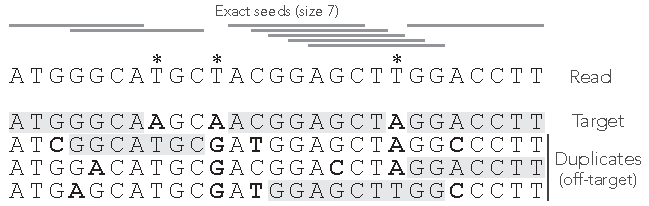
\includegraphics[scale=1]{exact_seed_example.pdf}
\caption{\textbf{Example of exact seeds.}
A sequenced DNA fragment (Read) is shown above its original form in the
genome (Target).}
\label{fig:exact_seed_example}
\end{figure}

Fig.~\ref{fig:exact_seed_example} also illustrates the seeding process
with exact seeds of size $\gamma=7$. It is clear that erroneous
nucleotides can also belong to exact seeds because they sometimes match
one of the duplicates. However, this is not the case of erroneous
nucleotides that are also mismatches for \emph{all} the duplicates, like
the second sequencing error in this example.

Thie middle of the read shows some cluttering where consecutive seeds
match consecutive sequences at the same location. This is typical for
exact seeds and constitutes a nuisance for the implementation. Indeed, it
is a waste of computer resources to discover matches in sequences that are
already in the candidate set. In addition, this seeding method is not
particularly sensitive~\cite{pmid11934743} so it is used only for specific
applications. Nevertheless, it will be extremely useful for the
development of the present theory.


\subsection{Skip seeds}

Skip seeds have a fixed size $\gamma$, but unlike exact seeds they cannot
start at every nucleotide. Instead, a fixed amount of nucleotides is
skipped between every seed. This is a way to reduce the amount of
overlapping matches at the same location, but the cost is a loss of
sensitivity. This seeding heuristic is used by
Bowtie2~\cite{pmid22388286}, where seeds have size $\gamma=16$ and fall
every 10 nucleotides (9 nucleotides are skipped between seeds).

\begin{figure}[h]
\centering
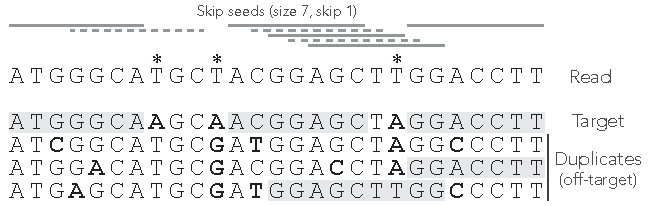
\includegraphics[scale=1]{skip_seed_example.pdf}
\caption{\textbf{Example of skip seeds.}
The sequences and the annotations are the same as in
Fig.~\ref{fig:exact_seed_example}, but here one nucleotide is skipped
betwen the seeds. In other words, seeds can never start on a nucleotide
with an even index. To highlight the difference with
Fig.~\ref{fig:exact_seed_example}, the missing seeds are represented by
dotted lines. Skipping nucleotides reduces the clutter at the center of
the read, but it also removes the only seed for the second duplicate.}
\label{fig:skip_seed_example}
\end{figure}

Fig.~\ref{fig:skip_seed_example} shows the seeding process on the read of
Fig.~\ref{fig:exact_seed_example} when using skip seeds instead of exact
seeds. Here the size is still $\gamma=7$ but 1 extra nucleotide is skipped
between seeds. This amounts to removing every other seed. The consequence
is that there are fewer overlapping matches at the center of the read, but
the only seed for the second duplicate was lost. This is a rather positive
outcome because there is one off-target location fewer in the candidate
set, but in general the same might happen to the target.

It is clear that skipping nucleotides reduces the sensitivity of the
seeding, but to what extent? One could test this empirically, but it
depends on the seed length, the amount of nucleotides that are skipped,
the error rate of the sequencer and the size of the reads. The present
theory will allow us to get the answer automatically.


\subsection{MEM seeds}

We will now focus on a seeding heuristic known as ``MEM seeding'' (where
MEM stands for Maximal Exact Match). This approach gives good empirical
results when mapping short reads (it is for instance the
strategy\footnote{To be exact, BWA-MEM uses SMEM seeds (Super Maximal
Exact Match seeds).} of the popular mapper BWA-MEM~\cite{li2013aligning})
but there is presently no theory to justify its performance. A deeper
understanding of MEM seeding would be useful to calibrate the
speed/accuracy trade-off of this heurisitic.

Before developing a formal theory, let us explain in more detail what
Maximal Exact Matches are and how MEM seeding works.

\begin{definition}
A Maximal Exact Match (MEM) seed is a subsequence of a read that is
present in the genome of interest and that cannot be extended --- either
because the read ends or because the extended subsequence is not in the
genome.
\end{definition}

Fig.~\ref{fig:MEM_example} shows a concrete example where a read is
aligned to candidate locations. The target (the true location of the
read) is first potential location. The locations below correspond to
duplicate sequences. The mismatches between the genome and the read are
highlighted in bold. The read has three errors indicated by stars, so
\texttt{T}, \texttt{T} and \texttt{C} should actually be \texttt{A},
\texttt{A} and \texttt{G} (\textit{i.e.} as in the target sequence).

\begin{figure}[h]
\centering
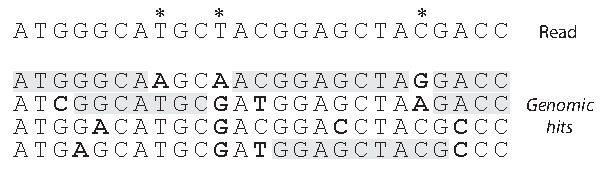
\includegraphics[scale=1]{MEM_example.pdf}
\caption{\textbf{Example of MEM seeds.}
A DNA fragment is sequenced with an imperfect instrument. It comes from
the top genomic location (Truth), but three errors were introduced
(indicated by stars). The sequence of the DNA fragment has three
duplicates at other genomic locations, shown below the target. Mismatches
between the read and the candidate sequence are highlighted in bold. MEM
seeds are indicated by grey boxes.}
\label{fig:MEM_example}
\end{figure}

The MEM seeds are indicated by grey boxes. Technically, they are part of
the read, but they are shown on the genome to highlight the position of
the match. One MEM seed cannot cover a smaller one (otherwise the smaller
would not be a MEM seed), but two consecutive MEM seeds can overlap, as in
the case of the frst two from the left. Note that overlapping MEM seeds
must match distinct sequences of the genome (otherwise neither of them
would be a MEM seed). Consecutive MEM seeds can also be disjoint, as in
the case of the second and the third from the left. In this case, they
must be separated by a nucleotide that is a mismatch against \emph{all}
the duplicates.


\section{Model and computational strategy}
\label{sec:symbolic}

\subsection{Sequencing error and duplications}

Now that this is clarified, we need to model the sequencing and the
duplication processes so that we can compute the probabilities of the
events of interest. We assume that the sequencing instrument has a
constant substitution rate $p$, and that insertions and deletions never
occur. When a substitution occurs, we assume that the instrument is
equally likely to output any one of the remaining three nucleotides. This
is a coarse-grain description of the error spectrum of the Illumina
technology~\cite{pmid21576222}.

Next, we assume that the target sequence has $N \geq 0$ duplicates, so
that there are $N$ off-target sequences. We further assume that
duplication happened instantaenously at some point in the past and that
all $N+1$ sequences diverge independently of each other at a constant
rate. In other words, we ignore the complications due to the genealogy of
the duplication events and we simply assume that at each position, any
given duplicate is identical to the target with probability $1-\mu$. If it
is not, we assume that the duplicate has any of the remaining three
nucleotides with equal probability (\textit{i.e.} each is found with
probability $\mu/3$).

Note that read errors are always mismatches against the target (because we
assume that the target is the true sequence), and they match each
off-target sequence with probability $\mu/3$. Correct nucleotides are
always a match for the target, and they match each off-target sequence
with probability $1-\mu$.


\subsection{Weighted generating functions}

The central object of analytic combinatorics is the generating function,
and for our particular purpose we will use a special kind known as
\emph{weighted generating function}.

\begin{definition}
\label{def:GF}
Let $\mathcal{A}$ be a set of combinatorial objects characterized by a
size in $\mathbb{N}$ and a weight in $\mathbb{R}^+$. The weighted
generating function of $\mathcal{A}$ is defined as

\begin{equation}
\label{eq:GF1}
A(z) = \sum_{a \in \mathcal{A}} w(a) z^{|a|},
\end{equation}
where $|a|$ and $w(a)$ denote the size and weight of the object $a$,
respectively. Expression (\ref{eq:GF1}) also defines a sequence $(a_k)_{k
\geq 0}$ such that 

\begin{equation*}
A(z) = \sum_{k=0}^\infty a_k z^k.
\end{equation*}

By definition $a_k = \sum_{a \in A_k}w(a)$, where $A_k$ is the class of
objects of size $k$ in $\mathcal{A}$. The number $a_k$ is the
total weight of objects of size $k$.
\end{definition}

To give a concrete example, if the probability of the symbol
$\downarrow_{/0}$ is $q$, the weighted generating function of a segment
containing only this symbol is $qz$. In our case, we are interested in the
weighted generating function of reads without good seeds, so that the
coefficient $a_k$ is equal to the probability that a read of size $k$ has
no good seed.

The motivation for introducing weighted generating functions is that
operations on combinatorial objects translate into operations on their
weighted generating functions. If $A(z)$ and $B(z)$ are the weighted
generating functions of two mutually exclusive sets $\mathcal{A}$ and
$\mathcal{B}$, the weighted generating function of $\mathcal{A} \cup
\mathcal{B}$ is $A(z) + B(z)$, as evident from expression (\ref{eq:GF1}).
Size and weight can be defined for pairs of objects in $\mathcal{A} \times
\mathcal{B}$ as $|(a,b)| = |a| + |b|$ and $w(a,b) = w(a)w(b)$. In other
words the sizes are added and the weights are multiplied.  With this
convention, the weighted generating function of the Cartesian product
$\mathcal{A} \times \mathcal{B}$ is $A(z)B(z)$. This simply follows from
expression (\ref{eq:GF1}) and from

\begin{equation*}
A(z)B(z) =
\sum_{a\in \mathcal{A}}w(a)z^{|a|} \sum_{b\in \mathcal{B}}w(b)z^{|b|}
= \sum_{(a,b) \in \mathcal{A} \times \mathcal{B}} w(a)w(b)z^{|a|+|b|}.
\end{equation*}

These two operations are all we need in order to compute the weighted
generating functions of the reads of interest. Addition corresponds to
creating a new family by merging reads from families $\mathcal{A}$ and
$\mathcal{B}$. Multiplication corresponds to creating a new family by
concatenating reads from families $\mathcal{A}$ and $\mathcal{B}$.

\subsection{Analytic representation}

The symbolic method is a strategy belonging to the general \emph{analytic
combinatorics} framework. The idea is to combine simple combinatorial
objects into more complex objects. Each combinatorial operation on the
objects corresponds to a mathematical operation on their weighted
generating functions. One can thus obtain the weighted generating function
of complex objects, and from there extract their probability of
occurrence.

The combinatorial construction of reads using the extended MEM alphabet
gives us a method to express their weighted generating function from the
simpler generating function of segments. More specifically, we can
describe complex sequences of segments through a so-called \emph{transfer
matrix} $M(z)$ that specifies which pairs of consecutive segments are
allowed and which are forbidden in the reads of interest.

The segment types are identified by their terminators arranged in a
predefined oder. The entry of $M(z)$ at coordinates $(i,j)$ is the
weighted generating function of segments with the $j$-th terminator that
can be inserted immediately after segments with the $i$-th terminator. The
entries of the matrix $M(z) + M(z)^2 + \ldots = M(z) \cdot (I-M(z))^{-1}$
are the weighted generating functions of the reads of all sizes using all
the allowed combinations of segments.

The entry of interest from $M(z)$ is the one that corresponds to the
terminators $\downarrow_{/0}$ and $|$ because it represents the reads of
any size whose first segment can be inserted after $\downarrow_{/0}$, and
whose last segment is terminated by $|$. Indeed, the $|$ terminator marks
the end of the read, so it must be the final symbol of every valid read.
As for the first segment, observe that all the segments that can follow
the $\downarrow_{/0}$ symbol are exactly those that can be at the frst
postion of the read\footnote{One could have introduced a special start
symbol. It is equivalent to an invisible $\downarrow_{/0}$ prepending
the reads.}.

In summary, the transfer matrix $M(z)$ contains the weighted generating
function of interest. Our next task is thus to specify $M(z)$.

More didactic descriptions of the strategy to compute seeding
probabilities using analytic combinatorics have been published
elsewhere~\cite{filion2017analytic,filion2018analytic}. The interested
readers can also discover more about analytic combinatorics in the
standard textbooks~\cite{flajolet2009analytic,sedgewick2013introduction}.


\subsection{Example 1: on-target exact seeds}
\label{sec:sample_exact}

We highlight the strategy above with an example that will turn out to be
central for the development of the theory. In addition, it is simple
enough to provide a gentle introduction to the general methodology. This
example was described in detail in~\cite{filion2017analytic} and
in~\cite{filion2018analytic}, but we repeat it here with a formalism that
fits the present manuscript.

The first step is to note that the nucleotide sequence of the read is
irrelevant. Indeed, the read has an on-target seed if and only if it
contains a stretch of $\gamma$ nucleotides without error. So the main step
is to recode the read as sequence of correct or erroneous nucleotides.

We define the mismatch alphabet $\mathcal{A}_0 = \{\square, |,
\Downarrow,\}$, where $\square$ represents a correct nucleotide,
$\Downarrow$ represents an erroneous nucleotide and $|$ is special symbol
appended after the last nucleotide to mark the end of the read.

This recoding allows us to segment the read in \emph{segments} defined as
a sequence of 0 or more symbols $\square$ followed by a symbol
$\Downarrow$. The last part of the read is called the tail and it is
terminated by the symbol $|$ instead of $\Downarrow$. The symbol $|$ does
not correspond to a nucleotide, it has size 0. This decomposition is
unique, so we can view a read as a sequence of segments with a tail,
instead of a sequence of nucleotides.

Fig.~\ref{fig:simple} shows an example of decomposition in segments.
On-target seeds cannot contain sequencing errors, therefore they must lie
inside a segment or inside the tail. So the size of the segments and of
the tail indicates whether the read contains an on-target seed.

\begin{figure}[h]
\centering
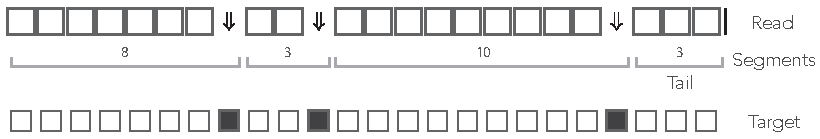
\includegraphics[scale=0.85]{sketch_simple.pdf}
\caption{\textbf{The mismatch encoding.}
A example read is represented in the match alphabet. The symbol
$\Downarrow$ represents a mismatch against the target sequence and
the symbol $\square$ represents a match.}
\label{fig:simple}
\end{figure}

The probability of occurrence of the symbol $\Downarrow$ is $p$, the error
rate of the sequencer, and the probability of occurrence of the symbol
$\square$ is thus $1-p = q$. Both symbols have size 1, so their respective
weighted generating function are $pz$ and $qz$. Using the rule for
concatenation, we see that the weighted generating function of a segment
with $m$ symbols $\square$ is $(qz)^mpz$. The symbol $|$ has size 0, so
the weighted generating function of a tail segment with $m$ symbols
$\square$ is $(qz)^m$.

The key insight is that reads without on-target seed correspond exactly
with the reads that are made of segments and tail with fewer than $\gamma$
symbols $\square$. The weighted generating function of such segments is
$pz \cdot \big( 1+qz+\ldots+(qz)^{\gamma-1} \big)$, and that of the tail
is $1+qz+\ldots+(qz)^{\gamma-1}$. This gives a construction plan that can
be encoded as a transfer matrix.

Since there are two kinds of bjects, the segments and the tails, the
dimensions of the transfer matrix are $2 \times 2$. A segment can be
followed by another segment or by the tail. The tail can be followed by
nothing. The expression of the transfer matrix $M(z)$ is thus
\begin{equation*}
\begin{blockarray}{ccc}
   & \scriptstyle{\Downarrow} & \scriptstyle{|} \\
\begin{block}{c[cc]}
\scriptstyle{\Downarrow} & pz \cdot \big( 1+qz+\ldots+(qz)^{\gamma-1}
\big)  & 1+qz+\ldots+(qz)^{\gamma-1} \\
\scriptstyle{|} & 0 & 0 \\
\end{block}
\end{blockarray}.
\end{equation*}

In this case, it is possible to compute $M(z) + M(z)^2 + \ldots = M(z)
\cdot (I-M(z))^{-1}$ directly and to extract the entry of interest.
Here it is the top right term because the read can start with a segment or
the tail (as if the read were prepended by an invisible segment), and it
must end with the tail. It is easy to check that the weighted generating
function is equal to
\begin{equation}
\label{eq:F}
\frac{1+qz+\ldots+(qz)^{\gamma-1}}
  {1-pz \big(1+qz+\ldots+(qz)^{\gamma-1} \big)}.
\end{equation}

The function above can be represented as a Taylor series $a_0 + a_1z +
a_2z^2 + \ldots$ By construction, $a_k$ is the quantity of interest,
\textit{i.e.} the probability that a read of size $k$ does not contain an
on-target seed, so we now need to extract those coefficients from
expression (\ref{eq:F}). There are several methods to do so, the one we
choose here is to build a recurrence equation to compute $a_k$ from the
previous terms of the series $a_0, a_1, \ldots, a_{k-1}$.

For this, we observe that equation (\ref{eq:F}) is equivalent to
\begin{equation*}
(1-qz) \left(1-pz \big(1+qz+\ldots+(qz)^{\gamma-1} \big)\right)
(a_0 + a_1z +a_2z^2 + \ldots) = 1-(qz)^\gamma.
\end{equation*}
Equating the terms of same degree on both side of the equal signs leads
to the following relationship between the coefficients of the series:
\begin{equation}
\label{eq:PE0}
a_k = 
\begin{cases}
1            &\quad\text{if } k < \gamma, \\
1 -pq^\gamma &\quad\text{if } k = \gamma, \\
a_{k-1} -pq^\gamma \cdot a_{k-\gamma-1} &\quad\text{otherwise.}
\end{cases}
\end{equation}

The term of interest can be computed recursively using expression
(\ref{eq:PE0}). This approach is very efficient because every iteration
involves at most one multiplication and one subtraction. Also, the default
floating-point arithmetic on modern computers gives sufficient precision
to not worry about numeric instability for the problems considered here
(we rarely need to compute those probabilities for reads above 500
nucleotides).

This example shows how the symbolic approach gives a non-trivial and yet
very simple method to compute the probability that a read of size $k$ does
not contain an on-target exact seed.


\subsection{Example 2: on-target skip seeds}

Another example that will turn out to be essential is to compute the
probability that a read contains no on-target skip seed. We tackle the
question with the same strategy as in the previous example, so we first
recode the reads using a more useful alphabet to solve this problem.

Once again, we need to know whether a nucleotide is a sequencing error,
but this time we also need to know its phase in the repeated cycles of
skipped positions. For this, we define the skip-$n$ alphabet
$\mathcal{A}_n = \{\square, |, \Downarrow_0, \Downarrow_1, \ldots,
\Downarrow_n \}$. As before, the symbol $\square$ represents a correct
nucleotide and the symbol $|$ is a terminator appended at the end of the
read. The symbols $\Downarrow_m$ ($m \in \mathbb{N}$) represent sequencing
errors and $m$ indicates the number of nucleotides till the next
non-skipped position (\textit{i.e.} $m=0$ for nucleotides immediately
before a non-skipped position and $m=n$ for nucleotides at a non-skipped
position).

The segments in this alphabet are defined as sequences of 0 or more
symbols $\square$ followed by any of the symbols $\Downarrow_m$. The tail
is again defined as a sequence of 0 or more symbols $\square$ followed by
the symbol $|$. Given that this decomposition is unique, we can again view
a read as a sequence of segments with a tail. The example of
Fig.~\ref{fig:simple} is showed again in Fig.~\ref{fig:skip}, where the
segments in the mismatch alphabet have been replaced by the segments in
the skip-3 alphabet,

\begin{figure}[h]
\centering
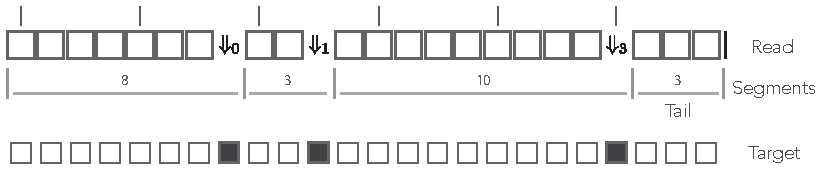
\includegraphics[scale=0.85]{sketch_skip.pdf}
\caption{\textbf{The skip encoding.}
Legend.}
\label{fig:skip}
\end{figure}

The probability of occurrence of a sequencing error is $p$ so the weighted
generating function of all the symbols $\Downarrow_m$ are identical and
equal to $pz$. The weighted generating function of the symbol $\square$ is
again $qz$, and so the weighted generating function of a segment with $m$
symbols $\square$ is again $(qz)^mpz$, and the weighted generating
function of a tail segment with $m$ symbols $\square$ is again $(qz)^m$.

Reads that do not contain any on-target skip seed can still contain
segments with $\gamma$ or more symbols $\square$, so this case is more
complex than the previous one. For instance, if there is a sequencing
error in phase $r$, the status of the next $r$ nucleotides does not have
any influence on the presence of an on-target seed. Indeed, there is no
on-target seed upstream of the error by construction, and the next seed is
scheduled to start $r$ nucleotides downstream of it, so the following
segment or tail can have up to $\gamma+r-1$ symbols $\square$. So in order
to enforce the absence of on-target seed, we have to adjust the maximum
size of the segments depending on the preceding terminator.

In the skip-$n$ alphabet, reads are composed of $n+2$ different kinds of
objects: the segments terminated by the $n+1$ symbols $\Downarrow_0,
\Downarrow_1, \ldots, \Downarrow_n$, plus the tail. The dimensions of the
transfer matrix are thus $(n+2) \times (n+2)$.

As mentioned above, after the $\Downarrow_r$ terminator, we can append
segments with up to $\gamma+r-1$ symbols $\square$. The terminators of
those $\gamma+r$ possible segments are distributed according to the laws
of the modulo $n+1$ arithmetic. For instance, if the next segment has no
symbol $\square$ then it is terminated by $\Downarrow_{r+1}$, but also if
it has $n+1$ symbols $\square$ (assuming $n+1 < \gamma$). Specifying the
transfer matrix thus involves a substantial amount of bookkeeping.

\begin{equation*}
\begin{blockarray}{cccccc}
   & \Dn{0} & \Dn{1} & \ldots & \Dn{n} & \nd \\
\begin{block}{c[ccccc]}
\Dn{0} & H_{0,0}(z) & H_{0,1}(z) & \ldots & H_{0,n}(z) & J_0(z) \\
\Dn{1} & H_{1,0}(z) & H_{1,1}(z) & \ldots & H_{1,n}(z) & J_1(z) \\
\vdots & \vdots & \vdots & \ddots & \vdots & \vdots \\
\Dn{n} & H_{n,0}(z) & H_{n,1}(z) & \ldots & H_{n,n}(z) & J_n(z) \\
\nd & 0 & 0 & \ldots & 0 & 0 \\
\end{block}
\end{blockarray}
\end{equation*}

\begin{eqnarray}
H_{r,s}(z) &=& pz \cdot (qz)^x \cdot \big( 1 + (qz)^{n+1} +
  \ldots + (qz)^{m(n+1)} \big), \\
\notag
  &\;& \text{where } x = r-s-1 \modulo{n+1},
  \text{ and } m = \left\lfloor
  \frac{\gamma+r-1-x}{n+1} \right\rfloor, \\
J_r(z) &=& 1 + qz + (qz)^2 + \ldots + (qz)^{\gamma+r-1}.
\end{eqnarray}

The transfer matrix is now too complex to compute a close expression
for $M(z)\cdot(I-M(z))^{-1}$. We return to the definition $M(z) + M(z)^2 +
\ldots$ and we observe that the terms $M(z)^{k+2}, M(z)^{k+3}, \ldots$
have no influence on the coefficients $a_0, a_1, \ldots, a_k$.

Indeed, a read of size $k$ has at most $k$ segments (plus one obligatory
tail). Since $M(z)^{s+1}$ contains the weighted generating functions of
reads with exactly $s$ segments and one tail, $a_k$ cannot depend on
$M(z)^{k+2}, M(z)^{k+3}$. More formally, we can prove by induction that
all the entries of $M(z)^k$ are divisible by $z^{k-1}$, showing that the
contribution of $M(z)^{k+2} + M(z)^{k+3} + \ldots$ to $a_0 + a_1z + \ldots
+a_kz^k$ is $0$.

So we can compute the matrix $M(z) + M(z)^2 + \ldots + M(z)^{k+1}$,
extract the entry of interest and then compute the terms of the Taylor
expansion up to order $k$. But we can do better. Since we are only
interested in the coefficients up to order $k$, we can perform all
algebraic operation on truncated polynomials of order $k$, \textit{i.e.},
we discard the coefficients of order $k+1$ or greater when multiplying two
polynomials.

But we can do even better. A read with $s$ segments contains $s$ errors.
Since read errors typically have a small probability of occurrence, all
the coefficients of $M(z)^{s+1}$ rapidly converge to $0$ as $s$ increases.
So instead of computing the matrix $M(z) + M(z)^2 + \ldots + M(z)^{k+1}$,
we can interrupt the summation after a certain power of $M(z)$ because the
terms become negligible.

The number of errors $X$ in a read of size $k$ has a Binomial
distribution $X \sim B(k,p)$. From~\cite{arratia1989tutorial} we can bound
the probabilities of the tail with the expression

\begin{equation}
\label{eq:bound}
Pr(X \geq s) \leq \exp \left( (s-k)\log \frac{k-s}{k(1-p)} -s\log
\frac{s}{kp} \right).
\end{equation}

Using the formula above, we can thus bound the probability that a read has
$s$ segments or more. We compute the matrices $M(z) + M(z)^2 + \ldots
+M(z)^{s+1}$ where the weighted generating functions have been replaced by
truncated polynomials and we extract the entry at the first column and the
last row. When the bound is lower than a set fraction $\varepsilon$ of the
smallest coefficient, we stop the computations. Typically $\varepsilon =
0.01$ so this method ensures that the probabilities that a read of size
$k$ has no good seeds are accurate to within 1\%.

\section{Exact seeds}

\subsection{Computing $P(E_0 \cap E_1)$}
\label{sec:cPE0E1}

The event $E_0 \cap E_1$ is that the read contains no match of size $\geq
\gamma$ for either the target or the first off-target sequence (here
``first'' refers to any fixed off-target sequence). We compute the
probability of this event with the strategy described in
section~\ref{sec:symbolic}: we first recode the reads using a different
alphabet and then we specify the transfer matrix of the reads that have no
match for any sequence. The powers of this matrix hold the weighted
generating function of interest, from which we extract the coefficients
that correspond to the terms $P(E_0 \cap E_1)$ for reads of different
sizes.

The reads are recoded as sequences of symbols from the so-called ``+/-
alphabet'' $\mathcal{A}_{+/-} = \{\square, |, \downarrow_{/1}^-,
\downarrow_{/2}^-, \ldots, \downarrow_{/1}^+, \downarrow_{/2}^+, \ldots,
\Downarrow\}$. The symbols $\downarrow_{/j}^-$ signify that the nucleotide
is a mismatch against the off-target sequence, the symbols
$\downarrow_{/j}^+$ signify that it is a mismatch against the target, and
the symbol $\Downarrow$ signifies that it is a mismatch against both. As
before, every other nucleotide is replaced by the symbol $\square$, and
the terminator $|$ is appended at the end of the read. We again define
reads as sequences of segments, except that now the terminators are the
symbols $\downarrow_{/j}^-$, $\downarrow_{/j}^+$, $\Downarrow$ and $|$.

The number $j$ in the symbol $\downarrow_{/j}^-$ indicates the relative
position of the last mismatch against the target. Likewise, the number $j$
in the symbol $\downarrow_{/j}^+$ indicates the relative position of the
last mismatch against the off-target sequence. In other words, the index
$j$ is the size of the match for the sequence that does not have a
mismatch. The terminators thus capture the local state of the read. For
instance the symbol $\downarrow_{/7}^-$ indicates that the nucleotide is a
mismatch against the off-target sequence, that it is a match for the
target, and that the six previous nucleotides were also a match for the
target.

\begin{figure}[h]
\centering
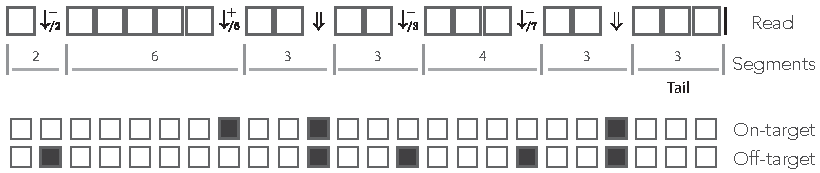
\includegraphics[scale=0.85]{sketch_dual.pdf}
\caption{\textbf{The +/- encoding.}
A example read is represented in the +/- alphabet. The symbols
$\downarrow_{/j}^-$ represent a mismatch against the off-target sequence,
the symbols $\downarrow_{/j}^+$ represent a mismatch against the target,
and the symbol $\Downarrow$ represent a mismatch against both. The index
$j$ is the number of matches since the last mismatch for the other
sequence. Note the presence of the terminator $|$ at the end of the read.
}
\label{fig:dual}
\end{figure}

We use the same error model as before: for every nucleotide, the read
differs from the target with a fixed probability $p$ and the sequences
differ from each other with a fixed probability $\mu$. With these
definitions, the probability of occurrence of the symbol $\square$ is $a =
(1-p)(1-\mu)$. Likewise, the collective probability of occurrence of the
symbols $\downarrow_{/j}^-$ is $b = (1-p)\mu$, that of the symbols
$\downarrow_{/j}^+$ is $c = p\mu/3$, and the probability of occurrence of
the symbol $\Downarrow$ is $d = p(1-\mu/3)$. It is easy to verify that
$a+b+c+d=1$.

These definitions allow us to specify the weighted generating function of
the segments. For instance, the weighted generating function of the
first segment of Fig.~\ref{fig:dual} is $(az)bz$, and that of the second is
$(az)^5cz$.

To specify the transfer matrix, we must ensure that we eliminate
the concatenations of two segments that would create a match of size $\geq
\gamma$ for any of the two sequences. After defining
\begin{equation*}
\begin{gathered}
r_i^+(z) = (az)^icz, \\
r_i^-(z) = (az)^ibz, \\
R_i(z) = \big( 1 + az + \ldots + (az)^i \big)dz, \\
F_i(z) = 1 + az + \ldots + (az)^i,
\end{gathered}
\end{equation*}
we can verify that the expression of the transfer matrix $L(z)$ is

\begin{equation*}
\begin{blockarray}{ccccccccc}
   & \scriptstyle{\Downarrow} & \scriptstyle{\downarrow_{/1}^+} & 
    \ldots & \scriptstyle{\downarrow_{\gamma-1}^+} &
    \scriptstyle{\downarrow_{/1}^-} & \ldots &
    \scriptstyle{\downarrow_{/\gamma-1}^-} & \scriptstyle{|} \\
\begin{block}{c[cccccccc]}
\scriptstyle{\Downarrow} & R_{\gamma-1}(z)  & r_0^+(z) & \ldots &
    r_{\gamma-2}^+(z) & r_0^-(z) & \ldots & r_{\gamma-2}^-(z) &
    F_{\gamma-1}(z) \\
\scriptstyle{\downarrow_{/1}^+} & R_{\gamma-2}(z) & & & & & & &
    F_{\gamma-2}(z) \\
\scriptstyle{\downarrow_{/2}^+} & R_{\gamma-3}(z) & & & & & & &
    F_{\gamma-3}(z) \\
\vdots & \vdots & & A(z) & & & B(z) & & \vdots \\
\scriptstyle{\downarrow_{/\gamma-1}^+} & R_0(z) & & & & & & & F_0(z) \\
\scriptstyle{\downarrow_{/1}^-} & R_{\gamma-2}(z) & & & & & & &
    F_{\gamma-1}(z) \\
\scriptstyle{\downarrow_{/2}^+} & R_{\gamma-3}(z) & & & & & & &
    F_{\gamma-2}(z) \\
\vdots & \vdots & & C(z) & & & D(z) & & \vdots \\
\scriptstyle{\downarrow_{/\gamma-1}^+} & R_0(z) & & & & & & & F_0(z) \\
\scriptstyle{|} & 0 & 0 & \ldots & 0 & 0 & \ldots & 0 & 0 \\
\end{block}
\end{blockarray},
\end{equation*}
where $A(z)$, $B(z)$, $C(z)$ and $D(z)$ are square matrices with
$\gamma-1$ rows/columns, that are defined as

\begin{equation*}
A(z) = 
\begin{blockarray}{cccccc}
   & \scriptstyle{\downarrow_{/1}^+} & \scriptstyle{\downarrow_{/2}^+} &
    \ldots & \scriptstyle{\downarrow_{/\gamma-2}^+} &
    \scriptstyle{\downarrow_{/\gamma-1}^+} \\
\begin{block}{c[ccccc]}
\scriptstyle{\downarrow_{/1}^+} & 0 & r_0^+(z) & \ldots &
    r_{\gamma-4}^+(z) & r_{\gamma-3}^+(z) \\
\scriptstyle{\downarrow_{/2}^+} & 0 & 0 & \ldots &
    r_{\gamma-5}^+(z) & r_{\gamma-4}^+(z) \\
\vdots & \vdots & \vdots & \ddots & \vdots & \vdots \\
\scriptstyle{\downarrow_{/\gamma-2}^+} & 0 & 0 & \ldots & 0 & r_0^+(z) \\
\scriptstyle{\downarrow_{/\gamma-1}^+} & 0 & 0 & \ldots & 0 & 0 \\
\end{block}
\end{blockarray},
\end{equation*}

\begin{equation*}
B(z) = 
\begin{blockarray}{cccccc}
   & \scriptstyle{\downarrow_{/1}^-} & \scriptstyle{\downarrow_{/2}^-} &
   \ldots & \scriptstyle{\downarrow_{/\gamma-2}^-} &
   \scriptstyle{\downarrow_{/\gamma-1}^-} \\
\begin{block}{c[ccccc]}
\scriptstyle{\downarrow_{/1}^+} & r_0^-(z) & r_1^-(z) & \ldots &
    r_{\gamma-3}^-(z) & r_{\gamma-2}^-(z) \\
\scriptstyle{\downarrow_{/2}^+} & r_0^-(z) & r_1^-(z) & \ldots &
    r_{\gamma-3}^-(z) & 0 \\
\vdots & \vdots & \vdots & \ddots & \vdots & \vdots \\
\scriptstyle{\downarrow_{/\gamma-2}^+} & r_0^-(z) & r_1^-(z) &
    \ldots & 0 & 0 \\
\scriptstyle{\downarrow_{/\gamma-1}^+} & r_0^-(z) & 0 & \ldots & 0 & 0 \\
\end{block}
\end{blockarray},
\end{equation*}

\begin{equation*}
C(z) = 
\begin{blockarray}{cccccc}
   & \scriptstyle{\downarrow_{/1}^+} & \scriptstyle{\downarrow_{/2}^+} &
    \ldots & \scriptstyle{\downarrow_{/\gamma-2}^+} &
    \scriptstyle{\downarrow_{/\gamma-1}^+} \\
\begin{block}{c[ccccc]}
\scriptstyle{\downarrow_{/1}^-} & r_0^+(z) & r_1^+(z) & \ldots &
    r_{\gamma-3}^+(z) & r_{\gamma-2}^+(z) \\
\scriptstyle{\downarrow_{/2}^-} & r_0^+(z) & r_1^+(z) & \ldots &
    r_{\gamma-3}^+(z) & 0 \\
\vdots & \vdots & \vdots & \ddots & \vdots & \vdots \\
\scriptstyle{\downarrow_{/\gamma-2}^-} & r_0^+(z) & r_1^+(z) & \ldots &
    0 & 0 \\
\scriptstyle{\downarrow_{/\gamma-1}^-} & r_0^+(z) & 0 & \ldots & 0 & 0 \\
\end{block}
\end{blockarray},
\end{equation*}

\begin{equation*}
D(z) = 
\begin{blockarray}{cccccc}
   & \scriptstyle{\downarrow_{/1}^-} & \scriptstyle{\downarrow_{/2}^-} &
    \ldots & \scriptstyle{\downarrow_{/\gamma-2}^-} &
    \scriptstyle{\downarrow_{/\gamma-1}^-} \\
\begin{block}{c[ccccc]}
\scriptstyle{\downarrow_{/1}^-} & 0 & r_0^-(z) & \ldots &
    r_{\gamma-4}^-(z) & r_{\gamma-3}^-(z) \\
\scriptstyle{\downarrow_{/2}^-} & 0 & 0 & \ldots &
    r_{\gamma-5}^-(z) & r_{\gamma-4}^-(z) \\
\vdots & \vdots & \vdots & \ddots & \vdots & \vdots \\
\scriptstyle{\downarrow_{/\gamma-2}^-} & 0 & 0 & \ldots & 0 & r_0^-(z) \\
\scriptstyle{\downarrow_{/\gamma-1}^-} & 0 & 0 & \ldots & 0 & 0 \\
\end{block}
\end{blockarray}.
\end{equation*}

The matrix $L(z)$ is relatively sparse and most non-zero entries are
monomials. In addition, the number of rows/columns is approximately
$2\gamma$, so the dimension of the matrix rarely exceeds 50. This means
that computing the powers of $L(z)$ is not prohibitive and we do not need
to design a Monte Carlo sampling scheme as we did before.

That being said, we do not need to compute all the powers up to $k$
because the terms vanish and become negligible after a certain iteration.
Indeed, the terms of $L(z)^n$ are the weighted generating function of the
reads without a match for either sequences and that contain exactly $n$
segments. Of those $n$ segments, $n-1$ are terminated by a mismatch
against at least one of the sequences. Following the rationale of
section~\ref{sec:extract}, we define $\tilde{p}$ as the upper bound on the
probability of a mismatch $\tilde{p} = \max\{b,c,d\}$, and updating
formula (\ref{eq:bound}) we bound the probability that a read of size $k$
contains $m = n-1$ or more mismatches

\begin{equation*}
Pr(X \geq m) \leq \exp \left( (m-k)\log \frac{k-m}{k(1-\tilde{p})} -m\log
\frac{m}{k\tilde{p}} \right).
\end{equation*}

The strategy is the same as in section~\ref{sec:extract}: we compute the
sum of matrices $L(z) + L(z)^2 + \ldots + L(z)^n$ where the weighted
generating functions have been replaced by truncated polynomials and we
extract the entry at the first column and the last row. When the bound is
lower than a set fraction $\varepsilon$ of the coefficient of $z^k$, we
stop the computations.

\subsection{Corollary: this title sucks}

The results of this section allow us to derive the probabilities of false
positives when using seeds of fixed size $\gamma$.

The complementary of the event $E_0$ is that the read contains at least
one match of size $\geq \gamma$ for the target, implying that there is a
seed for the target\footnote{This is the major difference with MEM seeds,
where the logical implication does not hold.}. With our assumptions this
means that the read is mapped to the correct location. The probability of
outcome $i.$, a true positive, is thus $1-P(E_0)$.

The event $E_0 \cap \ldots \cap E_N$ is that the read contains no match of
size $\geq \gamma$ for either the targer or any of the off-target
sequences. In other words, the probability of outome $iii.$, a false
negative, is $P(E_0 \cap \ldots \cap E_N)$.

The event $E_0 \cap (E_1 \cap \ldots \cap E_N)^c$ is that the read
contains no match of size $\geq \gamma$ for the target, but contains a
match of size $\geq \gamma$ for at least one of the off-target sequences.
In other words, the probability of outcome $ii.$, a false positive, is
$P(E_0) - P(E_0 \cap \ldots \cap E_N)$.

It is easy to see that the three probabilities sum to 1, as expected.
Below is a summary of the probabilities of interest.

\begin{eqnarray}
P(i.) &=& 1-P(E_0) \\
P(ii.) &=& P(E_0) \cdot \left( 1- \left( \frac{P(E_0
  \cap E_1)}{P(E_0)} \right)^N\right) \\
P(iii.) &=& P(E_0) \cdot \left( \frac{P(E_0 \cap E_1)}{P(E_0)} \right)^N
\end{eqnarray}

In the expressions above, we have used equation (\ref{eq:PE0E1}) to
highlight that these probabilities only depend on $P(E_0)$ and $P(E_0 \cap
E_1)$, which can be computed precisely as shown in sections~\ref{sec:cPE0}
and \ref{sec:cPE0E1}.

Note that the formulas also hold when the target has no duplicate
sequence. In this case, only outcome $i.$ and $iii.$ are possible, but
since $N=0$ we see that the second probability is 0, as expected.

\section{Skip seeds}


\begin{algorithm}[H]
\label{alg:mcmcskip}
\SetAlgoLined
\KwResult {Sample a read at random. Return 1 if the read contains a
good seed, otherwise return 0.}
  $\lambda \leftarrow 0$ \Comment*[r]{Current read size.}
  $s_+ \leftarrow 0$ \Comment*[r]{Current + match size.}
  $s_- \leftarrow 0$ \Comment*[r]{Current - match size.}
  \While {$\lambda < k$}{
    $i \leftarrow geom(a)-1$
                \Comment*[r]{Double-match nucleotides.}
    \If {$i > k-\lambda$}{
      $i \leftarrow k-\lambda$ \;
    }
    $s_+ \leftarrow s_+ + i$ \;
    $s_- \leftarrow s_- + i$ \;
    \If {$s_+ \geq \gamma$ or $s_- \geq \gamma$}{
      return 1 \;
    }
    $\lambda \leftarrow \lambda + i+1$ \;
    $r \leftarrow rand(0,1-a)$
                \Comment*[r]{Uniform random number.}
    \uIf {$r < b$}{
      $s_+ \leftarrow s_++1$ \;
      $s_- \leftarrow -\lambda \mod n+1$ \;
    }\uElseIf{$r < b+c$}{
      $s_+ \leftarrow -\lambda \mod n+1$ \;
      $s_- \leftarrow s_-+1$ \;
    }\uElse{
      $s_+ \leftarrow -\lambda \mod n+1$ \;
      $s_- \leftarrow -\lambda \mod n+1$ \;
    }
}
\eIf {$s_+ \geq \gamma$ or $s_- \geq \gamma$}{
  return 1 \;
}{
  return 0 \;
}
\end{algorithm}

\section{MEM seeds}

Before going further, we need to move a practical consideration out of the
way. It stands to reason that very short matches between the read and the
genome are uninformative. For instance, $99.7\%$ of all the possible
12-mers are present in the reference human genome, so an exact match of
size 12 or lower says nothing about the location of the DNA fragment. In
what follows, we will assume that subsequences of the read can only match
the original DNA sequence and/or its duplicates, but not the rest of the
genome. This will greatly simplify the exposition of the theory. We will
discuss how to relax this assumption in section~\ref{sec:short_MEMs}.

Observe that the rightmost MEM seed matches two genomic locations. This
case motivates the following definition, which will play an important role
for the development of the theory.

\begin{definition}
A \emph{strict} MEM seed has a single match in the genome.
A \emph{shared} MEM seed has several matches in the genome.
\end{definition}

Without surprise, the principle of MEM seeding is to use the genomic
matches of MEM seeds as candidate locations. Importantly, MEM seeds
shorter than a certain threshold $\gamma$ are ignored (in line with the
observation that short matches are uninformative). The parameter $\gamma$
is the tuning knob on the speed/accuracy trade-off. In
Fig.~\ref{fig:MEM_example} for instance, if $\gamma = 7$, there are three
candidate locations (the first, the second and the fourth) and if $\gamma
= 8$ there are only two (the first and the fourth).

Not every MEM seed makes the target a candidate location, so we introduce
the following terms to simplify the discussion.

\begin{definition}
Assume that the thresohld $\gamma$ is fixed. A \emph{good} seed is an
on-target MEM seed of size $\gamma$ or greater. In other words, the true
location is in the candidate set if and only if the read contains a
good seed.
\end{definition}

Compared to seeds of fixed size, MEM seeds have at least two
counter-intuitive (and undesirable) properties. The first is that there
are cases where there cannot be any good seed, even when changing
$\gamma$. Fig.~\ref{fig:full_masking_example} shows such an example. Even
though there is a single sequencing error, the read has no good seed.
Lowering $\gamma$ does not change this, so there is no way to discover the
true location (even though it is the best location).

\begin{figure}[h]
\centering
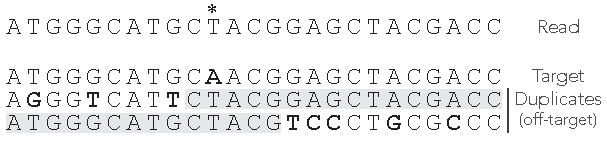
\includegraphics[scale=1]{full_masking_example.pdf}
\caption{\textbf{Issues with MEM seeds: inaccessible targets.}
The read, the MEM seeds and the sequences are represented as in
Fig.~\ref{fig:MEM_example}. The MEM seeds matching the two incorrect
locations at the bottom effectively hide the target, so it cannot
be discovered. This can occur even when the true location is the
best and when there is a single error on the read.}
\label{fig:full_masking_example}
\end{figure}

The second counter-intuitive property of MEM seeding is that shortening
a read can sometimes create a good seed. Fig.~\ref{fig:short_vs_long}
shows an example of this case. Again, there is no good seed, but there
would be one if the read were two nucleotides shorter on the right side.
Indeed, in this case there would be a shared MEM seed matching the first
and the second locations, provided $\gamma \leq 12$.


\begin{figure}[h]
\centering
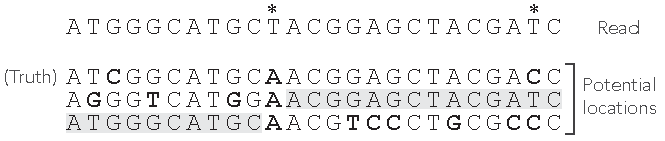
\includegraphics[scale=1]{short_vs_long_example.pdf}
\caption{\textbf{Issues with MEM seeds: too long reads.}
The read, the MEM seeds and the sequences are represented as in
Fig.~\ref{fig:MEM_example}. There would be a good seed (shared) if the
read were two nucleotides shorter. The true location is hidden by
the last two nucleotides.}
\label{fig:short_vs_long}
\end{figure}

These examples show that MEM seeds can perform worse than seeds of fixed
size. MEM seeds yield fewer candidates and therefore speed up the mapping
process, but the question is at what cost for accuracy? The theory
developed below will allow us to compute the probability that a read has
no good seed and thus that the true location is missed. This probability
is the key to evaluating and calibrating the MEM seeding heuristic.

We first expose a strategy to compute the probablity of true positives
(outcome $i.$), then show how to compute the probability of false
negatives (outcome $iii.$), and combine these two quantities to compute
the probability of false positives (outcome $ii.$). Finally, we provide a
computationally efficient method for estimating the parameters that are
necessary to estimate the probabilities of interest.


\section{Combinatorial construction}

In this section we represent reads as combinatorial ojects. The purpose of
this construction is to give a generative model of reads without good
seeds so that we can later compute their probability of occurrence.

\subsection{Hard and soft masking}

For each potential location including the target, we define the
\emph{match streak} at a given nucleotide as the number of nucleotides
since the last mismatch on the left, or since the beginning of the read.

\begin{definition}
At a given position of the read, an off-target sequence is a \emph{hard
mask} if its success streak is strictly longer than the match streak of
the target. An off-target sequence is a \emph{soft mask} if its has the
same match streak as the target.
\end{definition}

Fig.~\ref{fig:hard_vs_soft_masks} illustrates hard and soft masks with an
example. It is important to bear in mind that hard and soft masks depend
on the position of interest: a sequence can be a mask at the left end of
the read but not at the right end, or \textit{vice versa}. In the example
of Fig.~\ref{fig:full_masking_example}, every nucleotide of the read has a
hard mask, which is why the target cannot be discovered. In the example of
Fig.~\ref{fig:short_vs_long}, the middle sequence is a soft mask on the
right half of the read, but it turns into a hard mask two nucleotides
before the right end, which is why the target could be discovered if the
read were shorter.

\begin{figure}[h]
\centering
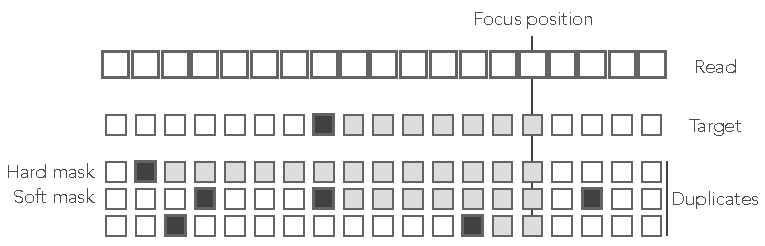
\includegraphics[scale=0.85]{hard_vs_soft_masks.pdf}
\caption{\textbf{Example of hard and soft masks.}
The nucleotides that do not match the read are reprsented as black boxes.
The nucleotides that contribute to the match streak are represented as
grey boxes. The remaining nucleotides are represented as open boxes. At
the given position, the match streak of the target is 7. The first
off-target is a hard mask because its match streak is $13>7$. The second
off-target sequence is a soft mask because its match streak is 7 like the
target. The third off-target sequence is not a mask because its match
streak is $2<7$.}
\label{fig:hard_vs_soft_masks}
\end{figure}

From the definition, we see that the last nucleotide of every strict
on-target MEM seed is always unmasked. Conversely, an unmasked nucleotide
always belongs to exactly one strict on-target MEM seed. Also, the last
nucleotide of every shared on-target MEM seed is always soft-masked, but a
soft-masked nucleotide does not always belong to a shared on-target MEM
seed.

Since hard and soft masks inform us about the positions of on-target
MEM seeds, we construct an alphabet that encodes the masking status of the
nucleotides.

\subsection{The MEM alphabet}

We recode the reads as sequences of letters from the so-called MEM
alphabet $\mathcal{A} = \{\square, |, \uparrow_{/1}, \uparrow_{/2},
\uparrow_{/3} \ldots, \downarrow_{/0}, \downarrow_{/1}, \downarrow_{/2},
\ldots\}$.

The symbols $\downarrow_{/m}$ indicate that the nucleotide is a sequencing
error and $m \geq 0$ is the number of off-target locations that
\emph{match} the nucleotide. Since a sequencing error is always a mismatch
against the target, the symbol $\downarrow_{/0}$ indicates that the
ncleotide is a mismatch against \emph{every} candidate.

The symbols $\uparrow_{/j}$ indicate a change in masking status: the
nucleotide is not masked but its left neighbor is. The index $j \geq 1$ is
the number of nucleotides since the last mismatch or since the beginning
of the read.

All the other nucleotides are represented by the $\square$ symbol.
Finally, the $|$ symbol is appended after the last nucleotide of the read.
It is an obligatory terminator that does not correspond to an actual
nucleotide.

Note that the numbers decorating $\uparrow$ and $\downarrow$ are different
in nature. In the case of the symbol $\downarrow$ it is an information
about the number of sequences matching the read; in the case of the symbol
$\uparrow$ it is the position of the previous sequencing error.
Fig.~\ref{fig:sketch_extended} shows the encoding of the read from
Fig.~\ref{fig:MEM_example} in the MEM alphabet.

\begin{figure}[h]
\centering
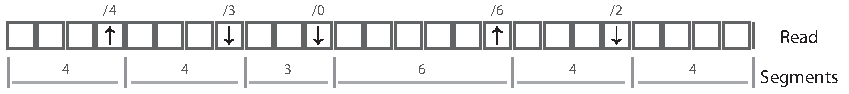
\includegraphics[scale=.85]{sketch_extended.pdf}
\caption{\textbf{The MEM encoding}.
The read of Fig.~\ref{fig:MEM_example} is represented in the MEM alphabet.
The arrows departing from those numbers help understand their meaning. The
$\downarrow$ symbol is decorated by the number of locations that match the
nucleotide. The $\uparrow$ symbol is decorated by the number of
nucleotides from the last error or from the beginning of the read. Also
note the presence of the terminator $|$ at the end of the read.}
\label{fig:sketch_extended}
\end{figure}

The MEM alphabet captures the masking status of the nucleotide as follows:
If we denote the number of off-targets as $N$, the symbol
$\downarrow_{/m}$ indicates that the nucleotide has $m$ hard masks and
$N-m$ soft masks. In addition, the symbols $\uparrow_{/j}$ indicate that
the nucleotide is unmasked.

In the MEM alphabet, strict on-target MEM seeds are the longest stretches
of symbols containing $\uparrow$ and not containing $\downarrow$. Indeed,
such a stretch matches the target, it matches the target only because it
contains at least one unmasked nucleotide (marked by $\uparrow$), and it
cannot be extended because it is flanked by sequencing errors or by the
ends of the reads. Note that there is exactly one symbol $\uparrow$ per
strict on-target MEM seed, and therefore that two symbols $\uparrow$ must
be separated by at least one symbol $\downarrow$.

Shared on-target MEM seeds are the longest stretches of $\square$ symbols
flanked by $\downarrow_{/0}$, or by the ends of the read. Indeed, such a
stretch is a MEM seed because it matches the target and it cannot be
extended ($\downarrow_{/0}$ is a mismatch against every sequence). Also,
it cannot be a strict on-target MEM seed because it does not contain the
$\uparrow$ symbol, so it must be shared.

\subsection{Reads as extended MEM segments}

Reads can be viewed as sequences of symbols, or as sequences of
\emph{segments}. For the purpose of constructing reads without good seeds,
the second point of view turns out to be essential.

\begin{definition}
\label{def:segment}
A segment is a maximal sequence of $\square$ symbols flanked on the right
side by one of the symbols $\uparrow_{/j}$, $\downarrow_{/m}$, or $|$. The
one and only segment flanked by $|$ is called the tail. It is the only
segment that can have size 0.
\end{definition}

In line with definition~\ref{def:segment}, the symbols $\uparrow_{/j}$,
$\downarrow_{/m}$ and $|$ are referrred to as \emph{terminators}.
Fig.~\ref{fig:sketch_segment} shows the segment representation of the read
from Fig.~\ref{fig:sketch_extended}.

\begin{figure}[h]
\centering
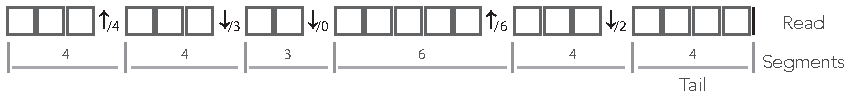
\includegraphics[scale=.85]{sketch_segments.pdf}
\caption{\textbf{The extended MEM segment encoding}.
The read from Fig.~\ref{fig:sketch_extended} is represented as a sequence
of segments. Each segment is terminated by either $\uparrow_{/j}$, or
$\downarrow_{/m}$ or $|$. The rightmost fragment is the tail. The numbers
below indicate the size of each segment in number of nucleotides.}
\label{fig:sketch_segment}
\end{figure}


We now have a representation of reads as sequences of segments. Only some
of these sequences are possible. For instance, a segment terminated by
$\uparrow$ cannot follow another. The task, however, is not to give a
construction of reads, but a construction of reads without good seeds. For
this, we need to introduce a new set of tools.



\section{The transfer matrix}
\label{sec:transfer_mat}



\subsection{Segments following $\uparrow_{/j}$}

A segment terminated by $\uparrow_{/j}$ is the beginning of an on-target
MEM seed of size at least $j$. The seed reaches the next sequencing
error or the end of the read, so the number of $\square$ symbols in the
next segment must be at most $\gamma-j-1$ and it must be terminated by a
$\downarrow$ symbol or by the tail terminator $|$.

On this segment, the matches between the read and the off-target sequences
are irrelevant. The weighted genearting function of each $\square$ symbol
is simply $qz$ ($q$ is the probability that the nucleotide is not an error
and $z$ marks objects of size $1$). The following definition will simplify
the notations.

\begin{definition}
The probability that a symbol is $\downarrow_{/m}$ given that the
nucleotide is a read error is
\begin{equation}
\label{eq:omega}
\omega_m = {N \choose m} \big(1 - \mu/3\big)^{N-m} \big(\mu/3\big)^m.
\end{equation}
\end{definition}

The weighted generating function of the $\downarrow_{/m}$ terminator is
thus $\omega_m pz$ (the probability of the symbol $\downarrow_{/m}$ is
$\omega_m p$ and $z$ marks objects of size $1$).

The entries of the transfer matrix that correspond to transitions from
$\uparrow_{/j}$ to other segments are now easy to find. The weighted
generating function of the segments terminated by $\downarrow_{/m}$
following a segment terminated by $\uparrow_{/j}$ is
\begin{equation}
\label{eq:D}
D_{j,m}(z) = \omega_m pz \sum_{i=0}^{\gamma-j-1} (qz)^i.
\end{equation}

And the weighted generating function of the tail segments following
segments terminated by $\uparrow_{/j}$ is
\begin{equation}
\label{eq:E}
E_j(z) = \sum_{i=0}^{\gamma-j-1} (qz)^i.
\end{equation}


\subsection{Segments following $\downarrow_{/m}$}

The symbol $\downarrow_{/m}$ signifies that the nucleotide has $m$ hard
masks and $N-m$ soft masks. If all the masks disappear before the first
read error, the next terminator will be a $\uparrow$ symbol, otherwise it
will be a $\downarrow$ symbol. We separate the cases based on the
terminator of the segment.

\subsubsection*{Case 1: the terminator is $\uparrow_{/i}$}

\begin{definition}
The probability that a given off-target sequence contains a mismatch in a
sequence of $i$ error-free nucleotides is
\begin{equation}
\label{eq:xi}
\xi_i = 1-(1-\mu)^i.
\end{equation}
\end{definition}

With this notation, the probability that at least one mask survives a
sequence of $i$ error-free nucleotides is thus $1-\xi_i^N$, and the
probability that there remains a mask at the $i-1$-th but not at the 
$i$-th error-free nucleotide is $\xi_i^N - \xi_{i-1}^N$. From this we
conclude that the weighted generating function of the segments terminated
by $\uparrow_{/i}$ following a segment terminated by $\downarrow_{/m}$ is
\begin{equation}
\label{eq:B}
B_i(z) = \Big( \xi_i^N-\xi_{i-1}^N \Big) (qz)^i.
\end{equation}

In the equation above, $q^i$ is the probability that there is no
sequencing error in $i$ nucleotides and $z^i$ marks objects of size $i$.
The fact that the reads have no good seeds imposes $i < \gamma$. Also note
that this expression is the same for all $\downarrow$ symbols; it does not
depend on $m$.

\subsubsection*{Case 2a: the terminator $|$ comes before the $\gamma$-th
nucleotide}

In this case there can be no good seed because the read terminates too
early. We must just enforce the condition that at least one of the $N$
masks survives until the end of the segment in order to exclude the
$\uparrow$ symbol. The weighted generating function is
\begin{equation*}
\sum_{i=0}^{\gamma-1} \Big(1 - \xi_i^N \Big) (qz)^i.
\end{equation*}

\subsubsection*{Case 2b: the terminator $|$ comes after the $\gamma$-th
nucleotide}

In this case, the soft masks do not hide the target: even if one of them
survives until the end of the read, there will be a good seed (shared in
this case). To make sure that the read has no good seed, we must enforce
the condition that at least one hard mask survives until the end of the
segment (which is impossible if $m = 0$). The weighted generating function
is
\begin{equation*}
\sum_{i=\gamma}^\infty \Big(1 - \xi_i^m \Big) (qz)^i.
\end{equation*}

Finally, the weighted generating function of the tail segments following
segments terminated by $\downarrow_{/m}$ is
\begin{equation}
\label{eq:C}
C_m(z) =
\sum_{i=0}^{\gamma-1} \Big(1 - \xi_i^N \Big) (qz)^i +
  \sum_{i=\gamma}^\infty \Big(1 - \xi_i^m \Big) (qz)^i.
\end{equation}

\subsubsection*{Case 3a: the terminator $\downarrow_{/n}$ comes before the
$\gamma$-th nucleotide}

In this case, there can be no good seed and we must only exclude the
$\uparrow$ terminator. The weighted generating function is
\begin{equation}
\omega_n pz \sum_{i=0}^{\gamma-1} \Big(1 - \xi_i^N \Big) (qz)^i.
\end{equation}

\subsubsection*{Case 3b: the terminator $\downarrow_{/n}$ comes after the
$\gamma$-th nucleotide}

This case is by far the most convoluted. Since the segment contains at
least $\gamma$ error-free nucleotides, we must ensure that it does not
contain a good seed. This will be the case if any of the two following
conditions is validated: $i)$ at least one hard mask covers all the
error-free nucleotides, or $ii)$ all the hard masks vanish but at least
one soft mask covers the whole segment (including the terminator).

The two conditions are mutually exclusive by construction. They are
graphically represented in the diagram below. The left panel corresponds
to case $i)$ and the panel to case $ii)$. The top row represents the
target, and the bottom rows represent off-target sequences (using the same
symbols as in Fig.~\ref{fig:MEM_example}).
\begin{inset}

\includegraphics{masks.pdf}
\end{inset}

Whenever a hard mask (here the first off-target sequence) covers the
nucleotides as shown in the left panel, there can be no good seed,
irrespective of the value of $\gamma$. The positions marked with a
question mark are irrelevant, they cannot change the fact that there is no
on-target MEM seed. If the hard masks vanish, as in the right panel, then
it all depends on the soft masks. If a soft mask covers the whole segment,
then there can be no good seed, irrespective of the value of $\gamma$.

Condition $i)$ has probability $\big(1 - \xi_i^m \big)$ and the
weighted generating function is thus
\begin{equation*}
\omega_n pz \sum_{i=\gamma}^\infty \Big(1 - \xi_i^m \Big) (qz)^i.
\end{equation*}

Condition $ii)$ is more convoluted, so we introduce some further
notations to solve this sub-case.
\begin{definition}
The probability that a given off-target sequence contains a mismatch in a
sequence of $i$ error-free nucleotides followed by an error is
\begin{equation}
\label{eq:eta}
\eta_i = 1-(1-\mu)^i\mu/3.
\end{equation}
\end{definition}

The probability of condition $ii)$ is
\begin{equation*}
\xi_i^m \Big(1 - \eta_i^{N-m} \Big),
\end{equation*}
but we need to break up this term among all the terminators
$\downarrow_{/n}$, ($0 \leq n \leq N$). For this, we decompose the sum on
the number of soft masks that run to the end of the segment, including the
terminator. The probability that there are $r \geq 1$ such soft masks is
\begin{equation*}
{N-m \choose r} (1 - \eta_i)^r \eta_i^{N-m-r}.
\end{equation*}

Each of them matches the nucleotide at the end of the segment, so the
total number of matches is $r$ plus the number of sequences that also
match the last nucleotide, among the remaining $N-m-r$ soft masks and $m$
hard masks.

Let us start with the $N-m-r$ that vanished somewhere in the segment. The
conditional probability that they match the last nucleotide given that
they vanish somewhere in the segment is $\mu/3 \cdot \xi_i / \eta_i$. The
conditional probability that they do not match it is $(1-\mu/3) / \eta_i$.
For the $m$ hard masks, the probability that they match the last
nucleotide given that they vanish somewhere in the segment is simply
$\mu/3$, and the probability that they do not match it is $1-\mu/3$.

The probability that the last nucleotide of the segment matches $n-r$ of
the $N-r$ masks that vanished before the terminator is
\begin{equation*}
\frac{(\mu/3)^{n-r}(1-\mu/3)^{N-n}}{\eta_i^{N-m-r}}
\psi_{i,m,n,r}\text{, where \;}
\psi_{i,m,n,r} = \sum_{q \geq 0}{m \choose q}{N-m-r \choose n-r-q}
\xi_i^{n-r-q}.
\end{equation*}


Finally, the probability that a total of $n$ off-target sequences match
the terminator and thus that the terminator is the symbol
$\downarrow_{/n}$ is
\begin{eqnarray*}
&\;& \sum_{r\geq1} {N-m \choose r}
(1 - \eta_i)^r (\mu/3)^{n-r} (1-\mu/3)^{N-n} \psi_{i,m,n,r} \\
&=& (\mu/3)^n(1-\mu/3)^{N-n} \sum_{r\geq1} {N-m \choose r}
  (1 - \mu)^{ri} \psi_{i,m,n,r} \\
&=& \omega_n \cdot \zeta_{i,m,n},
\end{eqnarray*}
where
\begin{equation}
\label{eq:zeta}
\zeta_{i,m,n} = \sum_{r\geq1} {N-m \choose r}
(1-\mu)^{ri} \psi_{i,m,n,r} \bigg/ {N \choose n}.
\end{equation}


The weighted generating function of the segments terminated by
$\downarrow_{/n}$ following segments terminated by $\downarrow_{/m}$ is
\begin{equation}
\label{eq:A}
A_{m,n} =
\omega_n pz \sum_{i=0}^{\gamma-1} \Big(1 - \xi_i^N \Big) (qz)^i + \omega_n
pz \sum_{i=\gamma}^\infty \Big(1 - \xi_i^m \cdot
(1- \zeta_{i,m,n}) \Big) (qz)^i.
\end{equation}

\subsection{Expression of the transfer matrix}
\label{sec:expression_of_M}

Collecting and arranging the results above, the final expression of the
transfer matrix $M(z)$ appears as
\begin{equation*}
\begin{blockarray}{cccccccc}
   & \dn{0} & \ldots & \dn{N} & \up{1} & \ldots & \up{\gamma-1} & \nd \\
\begin{block}{c[ccccccc]}
\dn{0} & A_{0,0}(z) & \ldots & A_{0,N}(z) & B_1(z) & \ldots &
    B_{\gamma-1}(z) & C_0(z) \\
\vdots & \vdots & \ddots & \vdots & \vdots & \ddots &
    \vdots & \vdots \\
\dn{N} & A_{N,0}(z) & \ldots & A_{N,N}(z) & B_1(z) & \ldots &
    B_{\gamma-1}(z) & C_N(z) \\
\up{1} & D_{1,0}(z) & \ldots & D_{1,N}(z) & 0 & \ldots & 0 & E_1(z) \\
\vdots & \vdots & \ddots & \vdots & \vdots & \ddots &
    \vdots & \vdots \\
\up{\gamma-1} & D_{\gamma-1,0}(z) & \ldots & D_{\gamma-1,N}(z) & 0 &
  \ldots & 0 & E_{\gamma-1}(z) \\
\nd & 0 & \ldots & 0 & 0 & \ldots & 0 & 0 \\
\end{block}
\end{blockarray}
\end{equation*}
where
\begin{gather}
\tag{\ref{eq:A}}
A_{m,n} =
\omega_n pz \sum_{i=0}^{\gamma-1} \Big(1 - \xi_i^N \Big) (qz)^i + \omega_n
pz \sum_{i=\gamma}^\infty \Big(1 - \xi_i^m \cdot
(1- \zeta_{i,m,n}) \Big) (qz)^i \\
\tag{\ref{eq:B}}
B_i(z) = \Big( \xi_i^N-\xi_{i-1}^N \Big) (qz)^i \\
\tag{\ref{eq:C}}
C_m(z) =
\sum_{i=0}^{\gamma-1} \Big(1 - \xi_i^N \Big) (qz)^i +
  \sum_{i=\gamma}^\infty \Big(1 - \xi_i^m \Big) (qz)^i \\
\tag{\ref{eq:D}}
D_{j,m}(z) = \omega_m pz \sum_{i=0}^{\gamma-j-1} (qz)^i \\
\tag{\ref{eq:E}}
E_j(z) = \sum_{i=0}^{\gamma-j-1} (qz)^i
\end{gather}
and where
\begin{gather}
\tag{\ref{eq:omega}}
\omega_m = {N \choose m} \big(1 - \mu/3\big)^{N-m} \big(\mu/3\big)^m \\
\tag{\ref{eq:xi}}
\xi_i = 1-(1-\mu)^i \\
\tag{\ref{eq:eta}}
\eta_i = 1-(1-\mu)^i\mu/3 \\
\tag{\ref{eq:zeta}}
\zeta_{i,m,n} = \sum_{r\geq1} {N-m \choose r}
(1-\mu)^{ri} \psi_{i,m,n,r} \bigg/ {N \choose n} \\
\notag
\psi_{i,m,n,r} = \sum_{q \geq 0}{m \choose q}{N-m-r \choose n-r-q}
\xi_i^{n-r-q}.
\end{gather}

The special case $N=0$ is worth describing in detail. This implies that
the target has no duplicate, so case $ii.$ is excluded (false positive),
and only cases $i.$ and $iii.$ are possible (true positive and false
negative, respectively). The transfer matrix $M(z)$ simplifies to the
extent that we can directly compute the weighted generating function of
reads without a good seed as
\begin{equation}
\tag{\ref{eq:F}}
F(z) = \frac{1+qz+\ldots+(qz)^{\gamma-1}}
  {1-pz \big(1+qz+\ldots+(qz)^{\gamma-1} \big)}.
\end{equation}

Expression (\ref{eq:F}) was shown in~\cite{filion2018analytic} to be the
weighted generating function of


\section{Computing the probabilities}
\label{sec:compute}

\subsection{Coefficient extraction}
\label{sec:extract}

The purpose of constructing the weighted generating function $F(z) = a_0 +
a_1z + a_2z^2 + \ldots$ is to extract the coefficient $a_k$, which
represents the probability that a read of size $k$ does not contain a
good seed.

$F(z)$ is the entry of the matrix $M(z) \cdot (I-M(z))^{-1}$ at the first
row and the last column, associated with terminators $\downarrow_{/0}$ and
$|$. The expression of $M(z)$ is too complex to compute this function
directly.


Instead, we return to the definition $M(z) \cdot (I-M(z))^{-1} =
M(z) + M(z)^2 + \ldots$ and observe that the terms $M(z)^{k+2},
M(z)^{k+3}, \ldots$ have no influence on the coefficients $a_0, a_1,
\ldots, a_k$.

Indeed, a read of size $k$ has at most $k+1$ segments\footnote{Each
segment contains a terminator, which has size 1, except the unique
terminator $|$, which has size 0.}. Since the entries of $M(z)^n$ are the
weighted generating functions of reads with exactly $n$ segments, $a_k$
cannot depend on $M(z)^{k+2}, M(z)^{k+3}$. More formally, we can prove by
induction that all the entries of $M(z)^k$ are divisible by $z^{k-1}$,
showing that the contribution of $M(z)^{k+2} + M(z)^{k+3} + \ldots$ to
$a_0 + a_1z + \ldots +a_kz^k$ is $0$.

So to extract the coefficients of $F(z)$ up to order $k$ we can compute
the matrix $M(z) + M(z)^2 + \ldots + M(z)^{k+1}$, isolate the entry at the
first row and the last column and then compute the terms of the Taylor
expansion up to order $k$.

But we can do better than that. Since we are only interested in the
coefficients up to order $k$, we can replace the infinite power series
of the terms $A_{m,n}(z)$ and $C_m(z)$ by their truncated versions where
we keep only the terms up to order $k$. Likewise, we perform all
algebraic operation on truncated polynomials of order $k$, \textit{i.e.},
we discard at every stage the coefficients of order $k+1$ or greater.

More formally, truncated polynomials are defined as polynomials whose
coeffients of degree greater than $k$ are 0. Multiplying two truncated
polynomials $P(z)$ and $Q(z)$ gives a truncated polynomial $R(z)$ whose
coefficients up to order $k$ are those of $P(z)Q(z)$. Using truncated
polynomials of order $k$, the entry of the matrix $M(z) + M(z)^2 + \ldots
+ M(z)^{k+1}$ at the first row and the last column directly provides the
coefficients of interest.

But we can do even better than that. A read with $n$ segments contains at
least $m=\lfloor{(n-1)/2}\rfloor$ errors. Indeed, two segments terminated
by $\uparrow$ cannot follow each other, so at least (approximately) half
of the segments must be terminated by $\downarrow$, which means that the
segment contains a read error. Since read errors typically have a small
probability of occurrence, all the coefficients of $M(z)^n$ rapidly
converge to $0$ as $n$ increases. So instead of computing the matrix $M(z)
+ M(z)^2 + \ldots + M(z)^{k+1}$, we can interrupt the summation after a
certain power of $M(z)$ because the terms become negligible.

The number of errors $X$ in a read of size $k$ has a Binomial
distribution $X \sim B(k,p)$. From~\cite{arratia1989tutorial} we can bound
the probabilities of the tail with the expression

\begin{equation}
\label{eq:bound}
Pr(X \geq m) \leq \exp \left( (m-k)\log \frac{k-m}{k(1-p)} -m\log
\frac{m}{kp} \right).
\end{equation}

Using the formula above, we can thus bound the probability that a read has
$n$ segments or more. We compute the matrices $M(z) + M(z)^2 + \ldots
+M(z)^n$ where the weighted generating functions have been replaced by
truncated polynomials and we extract $F_n(z)$, the entry at the first
column and the last row. When the bound is lower than a set fraction
$\varepsilon$ of the coefficient of $z^k$, we stop the computations.
Typically $\varepsilon = 0.01$ so this method ensures that the
probabilities that a read of size $k$ has no good seeds are accurate to
within 1\%.

This approach is feasible when the matrix $M(z)$ is small, but recall that
$M(z)$ has $N+\gamma+1$ rows/columns. Some sequences can have millions of
duplicates in plant and animal genomes (\textit{i.e.} $N > 10^6$), which
makes the computations with this method unfeasible because even a few
matrix multiplications are prohibitive. For large $N$, another method is
clearly needed.


\subsection{Monte Carlo sampling}
\label{sec:montecarlo}

The symbolic representation as MEM segments can be used for an efficient
method to sample reads. Instead of generating the nucleotides of the $N+1$
sequences one by one, one can generate a single sequence of MEM segments.
Since the number of segment does not depend on $N$, we can obtain a fast
Monte Carlo method to sample millions of reads and count the proportion
that contain a good seed.

The principle is to proceed in cycles of two steps. We first sample the
position of the next read error, which gives the position of the next
symbol $\downarrow$. The second step is to determine whether there is a
symbol $\uparrow$ before that. For this we sample the number of masks that
vanish before the symbol $\downarrow$. If they all vanish, the read
contains a good seed, provided the next read error is at a distance
greater than $\gamma$. Otherwise, the process is repeated until we
generate a good seed, or until the read has size $k$ or greater (in which
case it has no good seed).

The method is summarized by the algorithm below. It requires efficient
methods to generate random samples with a geometric distribution and a
binomial distribution. Sampling from a geometric distribution can be done
by computing the logarithm of a uniform $(0,1)$ random variable. Sampling
from a binomial distribution can be done by the method of
Kachitvichyanukul and Schmeiser~\cite{kachitvichyanukul1988binomial}.

\begin{algorithm}[H]
\label{alg:mcmc}
\SetAlgoLined
\KwResult {Sample a read at random. Return 1 if the read contains a
good MEM seed, otherwise return 0.}
  $\lambda \leftarrow 0$ \Comment*[r]{Current read size.}
  $m \leftarrow 0$ \Comment*[r]{Current number of hard masks.}
  \While {$\lambda < k$}{
    $i \leftarrow geom(p)-1$ \Comment*[r]{Error-free nucleotides.}
    \eIf {$i \geq k-\lambda$}{
      \eIf{$k-\lambda < \gamma$} {
        return 0\; }{
        $h \leftarrow binom(m,(1-\mu)^{k-\lambda})$
            \Comment*[r]{Surviving hard masks.}
        return 1 if $h = 0$, otherwise return 0\; }
    }
    {
      $h \leftarrow binom(m,(1-\mu)^i)$
          \Comment*[r]{Surviving hard masks.}
      $s \leftarrow binom(N-m,(1-\mu)^i \mu/3)$
          \Comment*[r]{Surviving soft masks.}
      \eIf {$ i \geq \gamma$ and $h = 0$ and $s = 0$}{
        return 1\;}{
        $m \leftarrow s + binom(N-s, \mu/3)$\;
        $\lambda \leftarrow \lambda + i+1$\;}
    }
 }
\end{algorithm}

In practice, we use a slightly modified version of this algorithm, that
returns the position of the good seeds if they are generated. This allows
us to estimate the probabilities for \emph{all} read sizes up to $k$. We
typically run this Monte Carlo sampling scheme 10,000,000 times, so that
we can estimate probabilities as low as $\sim1$ in 1 million.

The running speed depends on the error rate of the instrument $p$, but not
on the number of off-target sequences $N$. For values of $p$ around 0.01,
the running time for 10,000,000 iterations is $1$-$10$ seconds on current
hardware.

Algorithm~\ref{alg:mcmc} is a major result. It gives a compact solution to
the problem of estimating the probability that a read can be mapped when
using MEM seeds. The algorithm is also much faster than the naive approach
of sampling every nucleotide of every sequence, because it samples many
nucleotidea from \emph{all} the sequences at each iteration.

\section{False positives}

So far we have designed a method to estimate the probability that a
sequencing read contains a good seed. We referred to this as outcome $i.$
in section~\ref{sec:seedheur}. However, we are interested in the
probability that a read is mapped at an incorrect location, which is
outcome $ii.$

Computing the probability of outcome $ii.$ is hard, but we can compute the
probability that the read is not mapped at all, which is outcome $iii.$
The probability of outcome $ii.$ is then found by subtraction.

\subsection{Probability of outcome $iii.$}

Outcome $iii.$ implies that the read contains no seed at all, neither
on-target, nor off-target. This requires that there is no exact match of
size $\geq \gamma$ for \emph{any} sequence. Indeed, if it were the case,
then there would a MEM seed of size $\geq \gamma$ for at least one of the
sequences.

Let $E_0$ denote the event that there is no on-target match of size $\geq
\gamma$, and $E_j$ denote the event that there is no match of size $\geq
\gamma$ for off-target sequence $j$ ($1 \leq j \leq N$). We are thus
interested in computing $P(E_0 \cap \ldots \cap E_N)$. Since we assume
that the off-target sequences have evolved through the same mutagenesis
process and independently of each other, we can write

\begin{eqnarray}
\notag
P(E_0 \cap \ldots \cap E_N) &=&
  P(E_0) \cdot P(E_1 \cap \ldots \cap E_N | E_0) \\
\label{eq:PE0E1}
  &=& P(E_0) \cdot P(E_1 | E_0)^N =
  P(E_0) \cdot \left( \frac{P(E_0 \cap E_1)}{P(E_0)} \right)^N.
\end{eqnarray}

Expression (\ref{eq:PE0E1}) shows that we can compute the probability of
outcome $iii.$ from two quantities, namely $P(E_0)$ and $P(E_0 \cap E_1)$.

\subsection{Computing $P(E_0)$}
\label{sec:cPE0}

$P(E_0)$ is straightforward to evaluate because it involves a single
sequence. Methods to do this efficiently have been explained in detail
elsewhere~\cite{filion2018analytic}. Here we only give the recurrence
equation to compute $P(E_0)$. Assume that the probability of a sequencing
error $p$ is known, that $q = 1-p$, and that $a_k$ is the probability that
a read of size $k$ does not contain a match of size $\geq \gamma$ for the
target. This case was already treated in section~\ref{sec:example_exact}.

Knowing the size of the read and the error rate of the sequencing
instrument, we can thus compute $P(E_0)$ using expression (\ref{eq:PE0}).


\subsection{Probability of false positives}

For given values of the parameters $p$, $\mu$ and $N$, we can now compute
the probability of a false positive, which is outcome $ii$.

For this, we compute the probability of outcome $i.$, either by computing
the powers of $M(z)$ or by Monte Carlo sampling as explained in
section~\ref{sec:compute}. Next we compute the probability of outcome
$iii.$ using expression (\ref{eq:PE0E1}), where the terms are computed as
explained in sections~\ref{sec:cPE0E1} and \ref{sec:cPE0}.

When the target has no duplicate sequence, there can be no false positive
so this probability must be 0. In this case $N=0$ so according to formula
(\ref{eq:PE0E1}) outcome $iii.$ has probability $P(E_0)$. 

XXXX

XXXX

XXXX

XXXX

XXXX

XXXX

XXXX

XXXX

XXXX

XXXX

XXXX

XXXX

XXXX


\section{Estimating the parameters}
\label{sec:est}

So far we have assumed that we know all the specifications of the problem,
including the error rate of the instrument $p$, the number of off-target
sequences $N$, and their rate of sequence divergence $\mu$ (or more
accurately the probability that they differ from the target at every
nucleotide).

In general, $p$ is known from the vendor of the sequencing instrument, but
$N$ and $\mu$ can change for every read and they are usually unknown. We
thus need an estimation algorithm that can run fast enough that it does
not slow the mapping process. The main idea here is to use the backward
search, which is the method used to find the MEM seeds in the first place.

The backward search is a method that was first proposed by Ferragina and
Mazini~\cite{ferragina2000opportunistic} to identify exact matches between
a text query and an index. The query is extended one letter/nucleotide at
a time, and at each iteration the search returns the number of matches in
the index/genome. This is thus a very efficient method to identify MEM
seeds, because one can keep extending the query until there is no match in
the genome or until the end of the read.

What matters for us is that we can run the backward search at some
arbitrary position of the read. The $i$-th iteration returns the number
$N_i$ of matches in the genome for a query sequence of length $i$.
Ignoring sequencing errors and focusing only on the $N$ off-target
sequences, the probability that the count goes from $N_i$ to $N_{i+1}$ is

\begin{equation*}
P(N_{i+1}|N_i) = {N_i \choose N_{i+1}}
\mu^{N_i-N_{i+1}}(1-\mu)^{N_{i+1}}.
\end{equation*}

Assuming that there are $N = N_0$ duplicates and that we run $m$
iterations of the backward search, the probability of the observations
$(N_1, N_2, \ldots, N_m)$ is thus

\begin{equation*}
P(N_1, \ldots, N_m|N_0) = 
{N_0 \choose N_1 } \ldots {N_{m-1} \choose N_m }
\mu^{N_0-N_m}(1-\mu)^{N_1+\ldots+N_m}.
\end{equation*}

This is a familiar distribution in disguise: by defining $\Delta_i =
N_{i-1} - N_i$, the series of observations $(\Delta_1, \ldots, \Delta_m,
N_m)$ given $N_0$ has a multinomial distribution with parameters
$\big(\mu, \mu(1-\mu), \ldots, \mu(1-\mu)^{m-1}, (1-\mu)^m\big)$. More
specifically, the probability of observing the sequence $(\Delta_1,
\ldots, \Delta_m, N_m)$ given $N_0$ is

\begin{align*}
{N_0 \choose \Delta_1, \ldots, \Delta_m, N_m}
\mu^{\Delta_1}\big(\mu(1-\mu)\big)^{\Delta_2}
\ldots \big(\mu(1-\mu)^{m-1}\big)^{\Delta_m}(1-\mu)^{mN_m}.
\end{align*}

At that point, we need to bring back into the light the practical
consideration that short matches are uninformative. This implies that the
first iterations of the backward search say nothing about the number of
duplicates of the sequence. In practice, we are better off ignoring the
output of the first $n-1$ iterations by just discarding them. We observed
that running 30 iterations of the backward search and discarding the
output of the first 20 gives good results (\textit{i.e.} we set $n = 21$
and $m=30$).

Now, if $N_0, N_1, \ldots, N_{n-1}$ are missing, we obtain the probability
of observing $(\Delta_{n+1}, \ldots, \Delta_m, N_m)$ from the marginal
distribution as

\begin{align*}
\begin{split}
{N_0 \choose N_0-N_n, \Delta_{n+1}, \ldots, \Delta_m, N_m}
\big(1-(1-\mu)^n\big)^{N_0-N_n}
\big(\mu(1-\mu)^n\big)^{\Delta_{n+1}} \times
\ldots \\
\ldots \times
\big(\mu(1-\mu)^{m-1}\big)^{\Delta_m}(1-\mu)^{mN_m}.
\end{split}
\end{align*}

Now replacing again $\Delta_i$ by $N_{i-1}-N_i$, the log-likelihood can be
expressed as

\begin{equation}
\begin{split}
\ell = cst + \log \Gamma(N_0+1) - \log \Gamma(N_0-N_n-1)
+ (N_0-N_n) \log \big(1-(1-\mu)^n\big) + \\
(N_n-N_m) \log(\mu) + (nN_n + N_{n+1} + \ldots + N_m) \log(1-\mu).
\end{split}
\end{equation}

To estimate the parameters by maximum likelihood, we differentiate $\ell$
with respect to $N_0$ and with respect to $\mu$, then we equate both terms
to 0. We thus have to solve

\begin{gather}
\label{eq:psi}
\Psi(N_0+1)-\Psi(N_0-N_n+1) +
  \log\big( 1-(1-\mu)^n \big) = 0, \text{ and} \\
\label{eq:N0}
\frac{N_n-N_m}{\mu}
-\frac{nN_n + N_{n+1}+\ldots+N_m}{1-\mu} +
(N_0-N_n)\frac{n(1-\mu)^{n-1}}{1-(1-\mu)^n} = 0.
\end{gather}

In the expressions above, $\Psi(\cdot)$ is the digamma function, defined
as the derivative of $\log \Gamma(\cdot)$. We observe that equation
(\ref{eq:N0}) gives an expression of $N_0$ as a function of $\mu$ and of
the observations, namely

\begin{equation*}
N_0 = N_n +
\left(\frac{nN_n+N_{n+1}+\ldots+N_m}{1-\mu}-
\frac{N_n-N_m}{\mu} \right)
\frac{1-(1-\mu)^n}{n(1-\mu)^{n-1}}.
\end{equation*}

To find the maximum likelihood estimate of $\mu$, we can substitute this
expression in equation (\ref{eq:psi}), obtaining an equation depending on
$\mu$ and on the observations, which can be solved numerically. One can
then substitute the solution into equation (\ref{eq:N0}) to obtain the
estimate of the number of duplicate sequences $N_0$.

However, the estimations of $\mu$ and $N_0$ show large deviations from the
target values on simulated data. In practice, one does not need to know
the parameters with exquisite precision, so to avoid unrealistic
estimates, we pick the best $\mu$ from a short list of candidate values
(\textit{e.g.}, 0.02, 0.04 and 0.06). To do this, we choose a value
$\mu^*$ from the candidate set, we compute $N_0(\mu^*)$ from equation
(\ref{eq:N0}) and we evaluate $\ell$ with these values. Finally, we select
the $\mu$ that gives the higest value of $\ell$, and the estimate for
$N$ is set to $N_0(\mu)$.

Finding the estimates of $N$ and $\mu$ can be performed in negligible time
compared to running the backward search. We can repeat this method at
different areas of the read and finally average the estimates to get
reasonable values of $N$ and $\mu$ for the whole read. With this
information, we can compute the probability that the read has no good seed
using the methods presented above.

\section{Neglected practical considerations}

To keep the focus on the MEM seeding process, we have ignored some
practicalities that we now have to revisit in order to evaluate the
feasibility of our approach.

\subsection{Is the true location the best one?}
\label{sec:not_the_best}

So far we have assumed that the true location is also the best one, so
that it is always discovered when it is in the candidate set. But how
likely is it that the true location is not the best one, and thus that it
is virtually impossible to discover?

Obviously, it is possible that the target has an exact duplicate. When
that happens, the read cannot be mapped unambiguously, but this case is
relatively easy to detect, so the mapper can return a low confidence score
and thus avoid making an error.

From now we assume that the read has no strict duplicate. The probability
that the read of size $k$ has $m$ errors is
\begin{equation*}
{k \choose m}p^m(1-p)^{k-m}.
\end{equation*} 
A given duplicate has a better score if its Hamming distance from the read
is less than $k$. In a first order approximation, this happens if the
duplicate matches one of the $k$ errors, and also the $L-k$ correct
nucleotides. The probability of this even is
\begin{equation*}
m(1-\mu)^{k-m}\mu/3.
\end{equation*}

There are $N$ duplicates that evolve independently, so the probability
that one of them has a better score than the target is
\begin{equation*}
1-\left(1-m(1-\mu)^{k-m}\mu/3\right)^N \approx Nm(1-\mu)^{k-m}\mu/3.
\end{equation*}

Combining the first and the last expression, we find that the probability
that the target does not have the best score is approximately
\begin{equation}
\label{eq:not_the_best}
\sum_{m=0}^k {k \choose m}p^m(1-p)^{k-m} Nm\mu/3(1-\mu)^{k-m} = 
Nk p \left(1-\mu(1-p)\right)^{k-1}\mu/3.
\end{equation}

For instance, for reads of size $k=100$ with error rate $p=0.01$, where
the target has $N=5$ duplicates with divergence $\mu=0.05$ we obtain an
estimate close to $10^{-4}$. In comparison, the probability of a false
positive when using MEM seeds with a minimum size $\gamma=17$ is
approximately $4.4\cdot10^{-4}$.

The probability that the target does not have the best score is usually
small, but it is of the same order of magnitude as the probabilities of
false positives with MEM seeds. The reason is that a common source of
false positives are the cases when the target does not have the best
score. Indeed, in this case the target is much less likely to have a MEM
seed.

In short, the event that the true location is not the best one is already
incorporated in the false positive rate and we do not recommend further
updating the estimates. In the case that one is interested in this event
\textit{per se}, formula (\ref{eq:not_the_best}) gives an approximate
probability of its occurrence. When $\mu$ is unknown, we can replace it by
its worst case value $\mu = 1/qL$, where $q=1-p$. But $N$ must be known at
least approximately because the proability increases with $N$.

In summary, the case that the true location is not the best one has a
small but not negligible probability. It is partly redundant with the
false positives generated during the MEM seeding process, and therefore it
is not straightforward to adjust the estimates accordingly. We do not
adjust them at all and consider that this case is already implicitly
accounted for.

\subsection{MEM seeds for other sequences}
\label{sec:short_MEMs}

To simplify the problem, we have assumed that MEM seeds can match only the
target or one of its duplicates. In practice, MEM seeds that overlap a
sequencing error often match random locations of the genome instead of the
duplicates. When this occurs, the MEM seeds are typically small because 
the match is random.

We select MEM seeds of size at least $\gamma$, and it is important for the
validity of the theory that all the MEM seeds above the threshold are
considered candidate locations. If not, the estimates of the false
positive rate are off. The hope is that spurious MEM seeds are shorter
than $\gamma$ so that they are invisible, but this is not always the case.
And if they qualify, we need to verify them.

Such random hits can be problematic for two reasons: First, the time spent
verifying them is wasted. Second, they can cause false positives.
Fortunately, both issues can be addressed so that they do not constitute a
major problem.

To save time during the alignment phase, we can prioritize the seeds so
that the best hit is likely to be discovered first, allowing us to bail
out from other alignments as early as possible. We can even bound
the maximum quality of some candidates so that the alignment can be
skipped altogether. For instance, if we already have a candidate at
distance 1 from the read, there is no need to verify candidates from MEM
seeds in the middle of the read. Indeed, the hit must be at distance at
least 2 because there is a mismatch before the MEM seed and another one
after it.

These considerations depend on the implementation of the mapper so we will
not further develop them. What matters is that random hits do not have to
impose a significant burden on the time needed to verify the candidates.

The second issue is that random hits can generate false positives. Such
false positives happen when the read does not belong to the reference
genome, or when it contains so many errors that no proper MEM seed was
found. Since the hit is not homologous to the read, the alignment score is
essentially random. The upshot is that it is easy to detect.

Indeed, if the candidate location is random, mismatches occur with
probability 3/4. If it is the right location, mismatches occur with
probability $p$. We discard the MEM seed, which is an automatic match of
size at least $\gamma$. Say that there remains $L$ nucleotides and that
$m$ of them are mismatches for the candidate location. Using Bayes
formula, we find that the probability that the location is random given
the observed alignment score is
\begin{equation}
\label{eq:bayes}
\frac{1}{1 + 4^L(p/3)^mq^{L-m}(1-\beta)/\beta},
\end{equation}
where $q=1-p$ and $\beta$ is the prior probability that the hit is
random.

One may have information about the level of contamination, allowing to
choose a meaningful value for $\beta$. For instance, sequencing runs are
often spiked by foreign DNA such as the phiX genome or other. If these
reads are not filtered automatically, $\beta$ can be set to their expected
frequency. For sequences that belong to the reference genome, random hits
are rather rare because the read must contain so many error that neither
the target nor its duplicates were discovered. The value of $\beta$ is
much smaller in this case, but nevertheless difficult to estimate.

That being said, the value of $\beta$ has little importance in practice.
Say that a read generates a hit in the genome such that 33 nucleotides
need to be aligned (the alignment status of the others was already known
from the seeding step). If the hit is random there is a 99.99\% chance
that at least 15 are mismatches. If $p = 0.01$, the denominator of
expression (\ref{eq:bayes}) is approximately $1 +
4.3\cdot10^{-18}(1-\beta)/\beta$. So unless $\beta < 10^{-17}$, the
support for the hypothesis that the hit is random is overwhelming.

Conversely, if the hit is not random, there is a 99.99\% chance that 4 or
less are mismathes. In this case, the denominator is approximately
$1+6.8\cdot10^9(1-\beta)/\beta$, so unless $\beta > 1-10^9$, the support
for the hypothesis that the hit is not random is overwhelming.

In general, one does not need to worry about the value of $\beta$ because
random hits are extremely visible when $p$ is small. For instance, one can
choose $\beta=1/2$ so that the term $(1-/\beta)/\beta$ disappears in
expression (\ref{eq:bayes}).

Because the probability that the best candidate is a random sequence is
either very small or very large, it either has no influence on the
probability of false positive, or completely dominates it. For every read,
we thus take the maximum of this probability or the estimated probability
that MEM seeding returned a false positive.

In summary, MEM seeds in random sequences happen relatively frequently,
but it is possible to minimize their computational burden. Also, they
are no cause for concern regarding false positives because they can easily
be detected using Bayes formula.



\section{Discussion}

We have devised a method to compute the probability that the MEM seeding
heuristic fails and sets up the mapping process for a false positive. This
fills a gap of theoretical knowledge to understand and calibrate the
performance of the MEM seeding heuristic. The pillars of our strategy are
borrowed from analytic combinatorics~\cite{flajolet2009analytic,
sedgewick2013introduction}, even though we do not follow the standard
programme. Constructing generating functions usually serves the purpose of
finding their singularities in order to approximate the solution. In our
case, however, the weighted generating functions cannot be computed so
this strategy is not applicable.

To find the probabilities of interest in the absence of a fully specified
weighted generating function, we compute only the first terms using
iterative methods as in sections~\ref{sec:extract}, \ref{sec:cPE0} and
\ref{sec:cPE0E1}, or using Monte Carlo sampling as in
section~\ref{sec:montecarlo}. In this regard, the breakthrough is the
encoding of reads as MEM segments, which is a form of implicit Markov
imbedding~\cite{fu1994distribution}.

The method is general, but it is important to clearly state the
assumptions it depends on. First and most importantly, we have ignored
insertions and deletions. We assume that the sequencing errors are
substitutions only, which makes the method adapted to the Illumina
technology, but not to deletion-prone instruments such as the Oxford
Nanopore technology. We also assume that insertions and deletions never
occur among duplicated sequences. This is obviously incorrect, but our
initial tests with real data suggest that this is a minor impediment. On
real genomes, the estimations are only approximately correct and this is
but one of several simplifying assumptions. The theory is substantially
intrincate; insertions and deletions would make it intractable.
It is presently unclear how gracefully incorporate them in the theory.

The second assumption is that all the candidate locations with a MEM
seed of size $\geq \gamma$ are tested with the exact sequence alignment
algorithm, so that the best location is always discovered if it is in the
candidate set. This is not completely unrealistic, but it is important to
realize that for plant and animal genomes, a shared MEM seed may have tens
of thousands of hits. Therefore, most mappers impose a limit on the number
of alignments so the best hit may not be found even if it is in the
candidate set. This is again a minor impediment, since we can correct the
probability that the location is a false positive when only some
candidates have been tested.

The third assumption is that all the duplicate sequences evolve
independently of each other and at the same rate. This is again incorrect,
because duplication events can happen continuously, creating complex
ancestry relationships. It is possible to infer the ancestry using tree
reconstruction techniques, but it would be challenging to incorporate this
information in the present theory. The symbols of the MEM alphabet
implicitly assume that the sequences are exchangeable and the complexity
of the calculations explodes if it is not the case.

The last assumption is that MEM seeds can match only the target or one of
its duplicates. This is not the case but we have shown how to gracefully
deal with this in section~\ref{sec:short_MEMs}.

The Monte Carlo approach of algorithm~\ref{alg:mcmc} is relatively
straightforward, so one may wonder why the approach with weighted
generating functions is necessary at all. The only reason is precision. To
estimate the frequency of an event by Monte Carlo sampling, it must occur
at least a few times in the simulation. For instance, with 10 million
rounds of sampling, frequencies around $1/1,000,000$ or lower cannot be
measured accurately. When not interested in rare events, it is thus a
perfectly reasonable strategy to use only Monte Carlo sampling.

For $N < 20$, the probability that a read does not contain a good seed is
the smallest, so we need a method that is accurate in this range.
Fortunately, the transfer matrix method is fast in this regime because the
matrix $M(z)$ has few rows/columns.


The proposed methods are compliant with the demand for speed of the
mapping algorithms. One needs to compute the probabilities only once for a
given value of $N$ and $\mu$ (the error rate $p$ is known and constant).
For $N > 20$, the iterative method is usually prohibitive and we need to
use Monte Carlo sampling instead. The running time depends on the desired
number of iterations, on $p$ and on the size of the reads $k$. Since those
are constant throughout the sequencing run, the method always takes the
same time (around 1 second for reads of size $100$-$200$ nucleotides on
modern hardware). The values of $N$ and $\mu$ can be binned in intervals
of interest so that there are only around $100$ pairs for a total cost of
a few minutes per run. Considering that mappers can process at most
$10,000$ reads per second per core, the time of mapping a sequencing run
of 250 million reads is over 7 hours, two orders of magnitude larger than
the time required to estimate the probabilities of error.

In conclusion, we presented a practical solution to the problem of
estimating the probability of false positives when using MEM seeds. This
solution is adapted for mapping short reads sequenced with the Illumina
technology. Being able to calibrate the MEM seeding heuristic not only
allows the user to choose how to balance speed versus accuracy, but also
opens new applications. For instance, one can map reads from contaminated
samples in pools of closely related genomes (\textit{e.g.}, modern human
and Neanderthal) in order to assign the reads to the organism they belong
to. The probabilities of false positives give the right level of
confidence in the assignment.

More generally, the analytic combinatorics programme is a very powerful
tool to address problems in bioinformatics. Here we have seen how this
strategy can be useful even when the generating functions cannot be
computed. Using the same ideas, one could calibrate heuristics used in
other alignment methods, especially in expanding fields such as long-read
technologies.


\section*{Acknowledgements}

We thank Ruggero Cortini for suggesting Monte Carlo methods as a way to
tackle intractable cases. We acknowledge the financial support of the
Spanish Ministry of Economy and Competitiveness (‘Centro de Excelencia
Severo Ochoa 2013-2017’, Plan Nacional BFU2012-37168), of the CERCA
Programme~/~Generalitat de Catalunya, and of the European Research Council
(Synergy Grant 609989).


%---------------------------------------------------------------
%---------------------------------------------------------------

\bibliography{references,pubmed}
\bibliographystyle{unsrt}

%----------------------------------------------------------------

\end{document}

%gs -dNoOutputFonts -sDEVICE=pdfwrite -o out.pdf latex.pdf 
